\documentclass[]{scrartcl}
\usepackage[a4paper,left=2cm,right=3cm,top=2cm,bottom=2cm]{geometry}
\usepackage{svg}
\usepackage{graphicx}
\usepackage[dvipsnames]{xcolor}
\usepackage{minted}
\usepackage{tcolorbox}
\usepackage[spanish]{babel}
\usepackage{mdframed}
\usepackage{epigraph}
\usepackage{wrapfig}


\tcbuselibrary{minted}
\tcbuselibrary{breakable}

\definecolor{bashcodebg}{rgb}{0.85,0.85,0.85}

\newtcolorbox{notebox}{colback=SpringGreen!15!white,
colframe=SpringGreen!50!black}

\newtcolorbox{importantbox}{colback=RubineRed!25!white,colframe=RubineRed!75!black}

\newtcolorbox[auto counter]{exbox}[1][]{%
colback=red!5!white,colframe=red!75!black,
fonttitle=\bfseries,
title=Ejercicio \thetcbcounter: , #1}

\newtcblisting[auto counter]{cbox}[2][]{%
listing engine=minted,
minted language=c,
minted style=friendly,
minted options={mathescape,autogobble, framesep},
colback=TealBlue!5!white,colframe=TealBlue!75!black,
fonttitle=\bfseries,
listing only,
title=Snippet \thetcbcounter: #2, 
nameref=Snippet \thetcbcounter: #2,
#1}

\newminted[ccode]{c}{
  style=friendly,
  linenos=false,
  autogobble,
  fontsize=\footnotesize,
  bgcolor=gray!5,
  framesep=2mm,
  baselinestretch=1.2 % Adjust line height if needed
}

\newtcblisting[auto counter]{bashbox}[1][]{%
listing engine=minted,
minted language=bash,
minted style=friendly,
minted options={mathescape,autogobble, framesep},
colback=bashcodebg,
colframe=black!70,
fonttitle=\bfseries,
listing only,
#1}

\newtcbinputlisting[]{\bashinput}[2][]{%
listing file={#2},
listing engine=minted,
minted language=bash,
minted style=friendly,
minted options={autogobble, framesep},
colback=bashcodebg,
colframe=black!70,
fonttitle=\bfseries,
listing only,
#1}

\usepackage{colortbl} % para /color
\usepackage{hyperref} % Necesario para \url y \href
\usepackage{caption} % Para usar captionof
\captionsetup{labelformat=empty, hypcap=false}

\hypersetup{
    colorlinks=true,
    linkcolor=CadetBlue,
    filecolor=CadetBlue,      
    urlcolor=CadetBlue,
    }

\newcommand{\hl}[1]{\textcolor{magenta}{\textbf{\texttt{#1}}}}

%opening
\title{Guía de C - avanzada}
\subtitle{Arquitectura y Organización del Computador}
\date{}
\begin{document}


\maketitle

\section*{Estructuras}
\epigraph{\textit{Insanity consists of building major structures upon foundations which do not exist.}}

\subsection*{¿Qué es una estructura?}

\begin{importantbox}
  \centering
  Una estructura es una \textbf{colección de variables} de distintos tipos, agrupadas bajo un mismo nombre.
\end{importantbox}

Las estructuras son una forma de agrupar datos relacionados en un solo tipo de dato.
Por ejemplo, si quisiéramos representar un \textbf{punto} en el espacio 3D, podríamos usar una estructura que contenga tres variables de tipo \hl{float} (una para cada coordenada).
Podríamos definir una estructura \hl{punto} de la siguiente manera:

\begin{cbox}[unbreakable]{struct}
  #include <stdio.h>

  struct punto {
      float x;
      float y;
      float z;
  };
  int main() {
      struct punto p1;
      p1.x = 1.0;
      p1.y = 2.0;
      p1.z = 3.0;

      printf("punto: (%f, %f, %f)\n", p1.x, p1.y, p1.z);
      return 0;
  }
\end{cbox}

Podemos acceder a los miembros de una estructura usando el operador \hl{.} (punto) y tratar a esa variable como una variable normal. En el ejemplo, definimos una estructura llamada \hl{punto} que tiene tres campos: \hl{x}, \hl{y} y \hl{z}, todos de tipo \hl{float}. Luego, en la función \hl{main}, creamos una variable de tipo \hl{punto} llamada \hl{p1} y le asignamos valores a sus campos. Podemos decir, que \hl{struct punto} es un \textbf{tipo de dato compuesto} que agrupa tres variables de tipo \hl{float}.
Podemos definir estructuras anidadas, es decir, estructuras dentro de otras estructuras. Por ejemplo, si quisiéramos representar un \textbf{jugador} en un mapa, podríamos definir una estructura \hl{player} que contenga otra estructura \hl{punto} para representar su posición en coordenadas cartesianas:
\begin{cbox}[unbreakable]{struct}
  #include <stdio.h>

  struct punto {
      float x;
      float y;
  };

  struct player {
      char nombre[50];
      struct punto posicion;
  };

  int main() {
      struct player player1;
      player1.posicion.x = 1.0;
      player1.posicion.y = 2.0;

      printf("Posición del player1: (%f, %f)\n", 
              player1.posicion.x, 
              player1.posicion.y);
      return 0;
  }
\end{cbox}

Como se ve en el ejemplo, nada impide que definamos arrays dentro de las estructuras. Por otro lado, podemos definir estructuras anónimas, es decir, estructuras que no tienen un nombre específico. Esto puede ser útil para crear estructuras temporales:

\begin{cbox}[]{struct}
  #define NAME_LEN 50

  struct {
    int elo;
    char name[NAME_LEN + 1];
    int ranking;
  } player1;

  int main() {
    player1.elo = 2800;
    player1.ranking = 1;

    return 0;
  }
\end{cbox}

Esta estructura tiene tres campos: \hl{elo} , \hl{name} y \hl{ranking}. En particular, podemos ver que ese struct no tiene nombre (se le suele llamar \textit{anonymous struct}), solamente creamos una instancia de esa estructura anónima, llamada \hl{player1}. 
Su layout en memoria sería algo así:

\begin{center}
  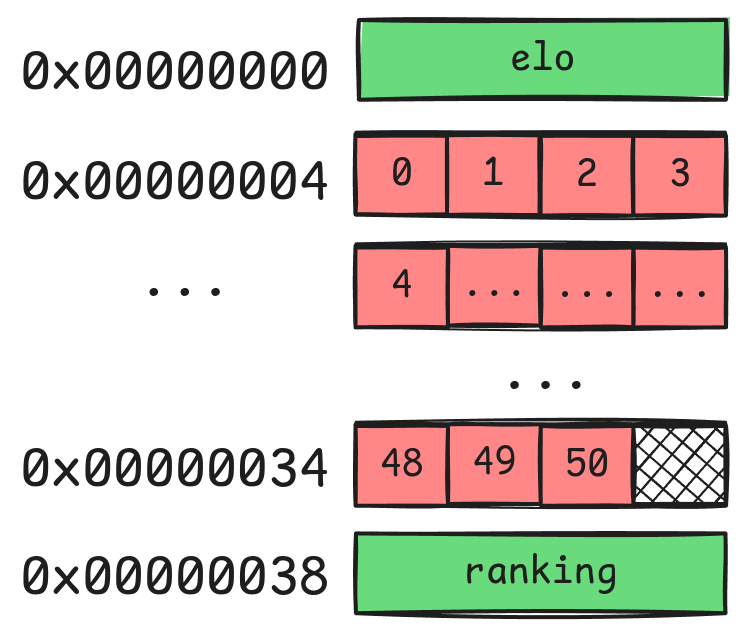
\includegraphics[scale=0.3]{./img/struct.png}  
  \captionof{table}{Struct en memoria}
  \label{fig:struct}
\end{center}

Notar el \textit{padding} que existe entre el array y el campo \hl{ranking}.
Esto se debe a que el compilador alinea los datos en memoria para optimizar el acceso a ellos. En este caso, el compilador decidió alinear el campo \hl{ranking} a un múltiplo de 4 bytes, lo que puede ser útil para mejorar la eficiencia del acceso a la memoria. Veremos en más detalle el tema de alineación y padding en la guia de Assembly. 

Podemos inicializar una estructura al momento de declararla, usando llaves:

\begin{cbox}[]{Inicialización de struct}
#define NAME_LEN 50

struct player{
  int elo;
  char name[NAME_LEN + 1];
  int ranking;
};

struct player player1 = { 2800, "Magnus Carlsen", 1 },
struct player player2 = { 2700, "Fabiano Caruana", 2 };

\end{cbox}

En este momento, es conveniente mencionar el keyword \hl{typedef}, que nos permite definir un nuevo tipo de dato basado en un tipo existente. El nuevo tipo también se conoce por el nombre de \textbf{type alias}. 
Esto es útil para simplificar la declaración de estructuras y hacer el código más legible. 

\begin{cbox}[]{typedef}
typedef float real_t;
typedef int quantity_t;
typedef unsigned long int size_t; // en <stdint.h>
typedef uint32_t vaddr_t; // direccion virtual.
typedef uint32_t paddr_t; // direccion fisica.
\end{cbox}

Notar como primero viene el tipo original y luego el nuevo tipo.

En el siguiente fragmento definimos una estructura y le asignamos un alias \hl{player\_t} para poder usarlo más fácilmente en el resto del código. Además, notar el tipo de inicialización alternativa de \hl{player3}:

\begin{cbox}[]{typedef de struct}
#define NAME_LEN 50

typedef struct {
  int elo;
  char name[NAME_LEN + 1];
  int ranking;
} player_t;

player_t player1 = { 2800, "Magnus Carlsen", 1 },
player_t player2 = { 2700, "Fabiano Caruana", 2 };
player_t player3 = { .name = "Hikaru Nakamura", 
                     .ranking = 3, 
                     .elo = 2600}; //forma alternativa
\end{cbox}

Por otro lado, la operación asignación \hl{=} en \hl{struct} produce una copia de la estructura completa.

\begin{cbox}[]{miembros}
player_t magnus = { 2800, "Magnus Carlsen", 1 },
player_t faustino;

printf("Elo: %d\n", magnus.elo);
printf("Name: %s\n", magnus.name);
printf("Ranking: %d\n", magnus.ranking);

magnus.elo = 2700;
magnus.ranking--;

faustino = magnus; // copia de estructura
\end{cbox}

Las estructuras pueden pasarse a funciones como argumentos y también pueden ser devueltas como valores de retorno.

\begin{cbox}[]{struct como argumento y valor de retorno}

player_t get_player(void) {
  player_t player = { 3000, "Bobby Fischer", 1 };
  return player;
}

void print_player(player_t player) {
  printf("Elo: %d\n", player.elo);
  printf("Name: %s\n", player.name);
  printf("Ranking: %d\n", player.ranking);
}

\end{cbox}

Notar que pasar estructuras grandes de esta manera puede ser ineficiente, ya que se copian todos los datos de la estructura. En su lugar, se suele usar punteros a estructuras, que son más eficientes. Lo veremos más adelante.

Nada impide que armemos un array de estructuras, como el siguiente:

\begin{cbox}[]{array de struct}
typedef struct {
  char* pais;
  int code;
} dials_code_t;

dials_code_t country_codes[] = {
  {"Argentina", 54},
  {"Brasil", 55},
  {"Chile", 56},
  {"Uruguay", 598}
};

printf("Código para Argentina: %d\n", country_codes[0].code);
\end{cbox}

La inicialización puede ser parcial también, como en el siguiente ejemplo:

\begin{cbox}[]{Inicialización de array de struct}
dials_code_t country_codes[100] = {
  [0] = {"Argentina", 54},
  [1] = {"Brasil", 55},
  [2] = {"Chile", 56},
  [3].pais = "Uruguay", [3].code = 598,
  // ... el resto se inicializa en 0
};
\end{cbox}

\begin{exbox}
  Definir una estructura \hl{monstruo\_t} que contenga los siguientes campos:
  \begin{itemize}
    \item \hl{nombre} (string)
    \item \hl{vida} (entero)
    \item \hl{ataque} (double)
    \item \hl{defensa} (double)
  \end{itemize}
  Luego, inicializar un array de monstruos y mostrar por pantalla el nombre y la vida de cada uno de ellos.
\end{exbox}

\begin{exbox}
  Definir una función \hl{evolution} que reciba un \hl{monstruo\_t} y devuelva un nuevo monstruo con los mismos atributos, pero con el ataque y defensa aumentados en 10. Luego, usar esta función para evolucionar un monstruo y mostrar por pantalla sus atributos antes y después de la evolución.
\end{exbox} 

\newpage
\section*{Punteros}

\epigraph{\textit{Paradox is a pointer telling you to look beyond it. If paradoxes bother you, that betrays your deep desire for absolutes. The relativist treats a paradox merely as interesting, perhaps amusing or even, dreadful thought, educational.}}

\subsection*{¿Qué es un puntero?}

\begin{importantbox}
  \centering
  Un puntero es una \textbf{variable que almacena una dirección de memoria}.
\end{importantbox}

\begin{center}
  
\includegraphics[scale=0.1]{./img/lionelhutz-contract.png}  
  \label{fig:simpsons-puntero}
\end{center}

En la guía anterior mencionamos al pasar que uno de los tipos nativos de C es el \textbf{puntero}, tipado \hl{int*}, \hl{char*}, \hl{void*}, etc.

\begin{center}
  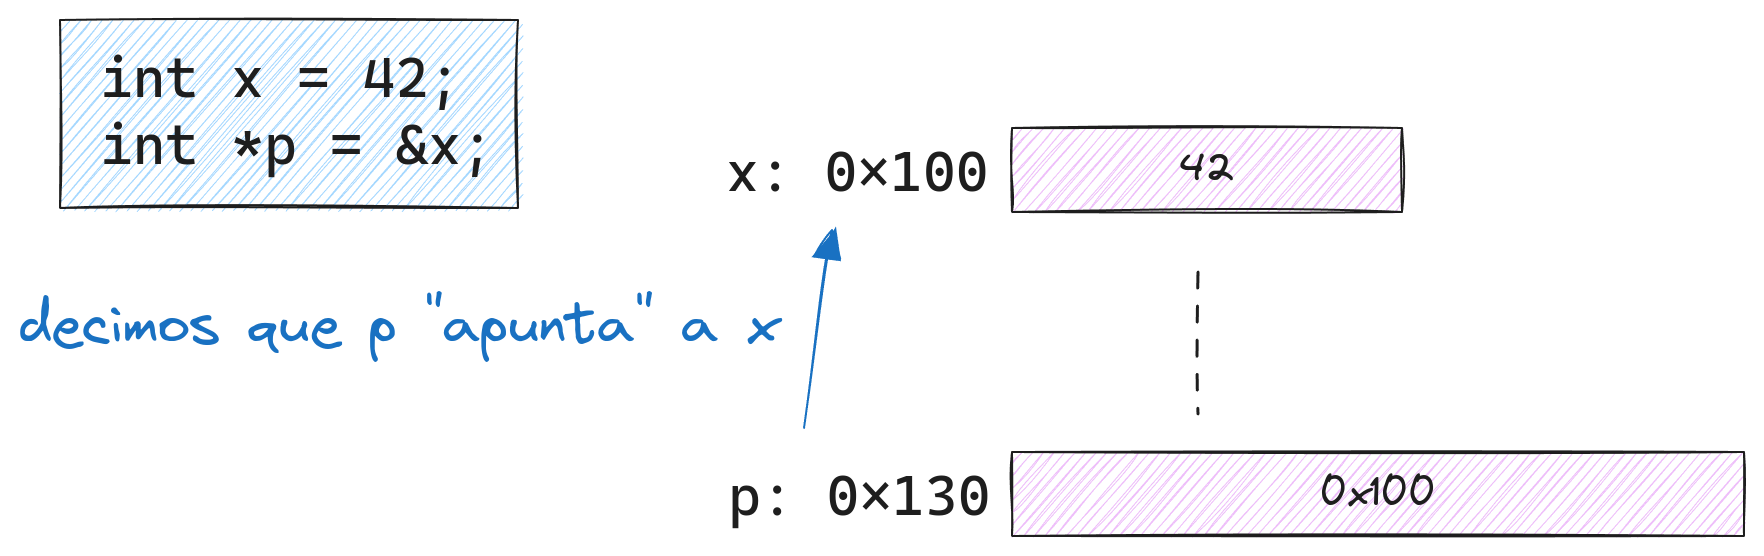
\includegraphics[scale=0.2]{./img/pointer.png}  
  \label{fig:simpsons-puntero}
\end{center}

Comencemos mirando el siguiente código:

\begin{cbox}[unbreakable,label=sni:xp,nameref={Snippet \ref{sni:xp}}]{}
  #include <stdio.h>

  int main(){
      int x = 42;
      int *p = &x;
  
      printf("Direccion de x:  %p Valor: %d\n", (void*) &x, x);
      printf("Direccion de p: %p Valor: %p\n", (void*) &p, (void*) p);
      printf("Valor de lo que apunta p: %d\n", *p);
  }
\end{cbox}

\begin{exbox}[label=ejercicio1]
  Sin correr el código, responder:
  \begin{itemize}
    \item ¿Cuál es la diferencia entre \texttt{x} y \texttt{p}? ¿Y entre \texttt{x} y \texttt{\&x}? ¿Y entre \texttt{p} y \texttt{*p}?
    \item ¿Qué valores creen que se van a imprimir por terminal?
  \end{itemize}
\end{exbox}

\begin{exbox}[label=ejercicio2]
  Compilar y ejecutar el código. 
  ¿Qué valores se imprimieron?
  ¿Qué creen que significan?
\end{exbox}

Para responder estas preguntas, es \textbf{clave} que entendamos como se organiza la memoria en C.

Al final del día, la memoria no es más que una tira de \textbf{bits} (1/0).
Pero usualmente queremos trabajar con variables con más valores que solo 0 y 1\footnote{Tener memorias del tamaño que utilizamos hoy, direccionables con granularidad de bit sería caro y dificultoso de implementar a nivel hardware. Este post de quora da una intuición al respecto \url{https://www.quora.com/Why-do-memory-addresses-use-the-unit-of-byte-instead-of-bit}.}, por lo que hoy en día usamos a la memoria como si fuera una tira de \textbf{bytes}, que son grupos de \textbf{8 bits}.

Entonces, desde ahora, pensemos a la memoria como una \textbf{tira de bytes contiguos}.
Vamos a poder acceder a cada uno de estos bytes individualmente, porque cada uno tiene una \textbf{dirección única} que lo identifica.

Llamamos \textbf{puntero} a una variable que guarda la dirección de un valor en memoria. Por ejemplo, si la memoria de la dirección \texttt{0xF0} (hexadecimal) a \texttt{0xF8} tiene esta pinta:
%
\begin{center}
  \noindent \makebox[\textwidth]{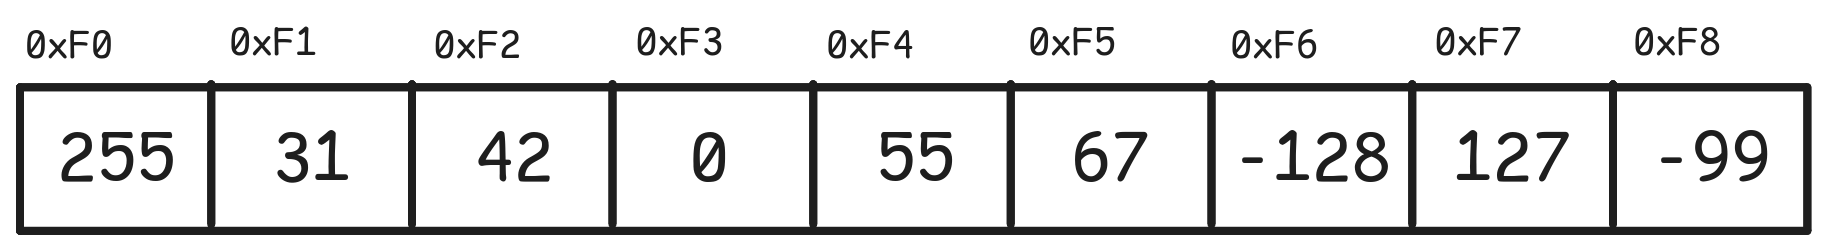
\includegraphics[width=0.5\paperwidth]{./img/memoria_bytes.png}}
  \label{fig:tira-memoria}
\end{center}
%
Podríamos declarar las siguientes variables:
\begin{cbox}[unbreakable]{}
  #include <stdio.h>
  #include <stdint.h>

  int main(){
    uint8_t *x = (uint8_t*) 0xF0;
    int8_t *y = (int8_t*) 0xF6;

    printf("Dir de x: %p Valor: %d\n", (void*) x, *x);
    printf("Dir de y: %p Valor: %d\n", (void*) y, *y);

    //Devolverá:
    //  Dir de x: 0xF0 Valor: 255
    //  Dir de y: 0xF6 Valor: -128
  }
\end{cbox}

\begin{exbox}[label=ejercicio3]
  ¿Por qué \texttt{x} e \texttt{y} tienen distintos tipos? ¿Qué representan?
\end{exbox}

Si intentan ejecutar ese código, probablemente el programa falle con un error de tipo \texttt{Segmentation fault (core dumped)}.
En nuestra computadora, la memoria esta siendo usada por varios componentes y es estadísticamente imposible que las direcciones \texttt{0xF0} a \texttt{0xF8} tengan los valores que usamos en este ejemplo.
De hecho, las direcciones \texttt{0xF0} a \texttt{0xF8} de memoria probablemente no estén a nuestro alcance porque seguramente las esté usando otro proceso (por ende ocurre un \texttt{Segmentation Fault}).

Si queremos una tira contigua de bytes como la mostrada en la imagen, necesitamos declararla.
Para eso, ¡podemos usar arrays! Como vimos en la guía anterior.

\begin{exbox}[label=ejercicio4]
  Completar los ?? en el siguiente código:

  \begin{cbox}[unbreakable]{}
    #include <stdio.h>
    #include <stdint.h>

    int main(){
        int8_t memoria[??] = ??;
        uint8_t *x = (uint8_t*) ??;
        int8_t *y = ??;

        printf("Dir de x: %p Valor: %d\n", (void*) x, *x);
        printf("Dir de y: %p Valor: %d\n", (void*) y, *y);
    }
  \end{cbox}

  \textbf{Pista:} ¿Para qué sirve el operador \texttt{\&}? Revisar los ejemplos de código anteriores o ver la sección \nameref{sec:operadores}.
\end{exbox}

Claramente, podemos usar el puntero, no solo para leer el valor de una dirección de memoria, sino también para escribir en ella.

\begin{cbox}[]{Escritura a través de puntero}
  #include <stdio.h>

  int main(){
      int x = 42;
      int *p = &x;
  
      printf("x: %d\n", x);
      *p = 200;
      printf("x: %d\n", x);
  }
\end{cbox}

\begin{bashbox}
x: 42
x: 200
\end{bashbox}

\subsection*{Declaración vs Desreferencia} 
\label{sec:operadores}

Habrán visto en los ejemplos hasta ahora que al trabajar con punteros contamos con dos operadores principales: \hl{*} y \hl{\&}.
Definamos propiamente:

\begin{itemize}
  \item \hl{*}: se usa en dos situaciones
  \begin{itemize}
    \item Al \textbf{declarar} un puntero: indica que la variable siendo declarada es un puntero al tipo indicado.
    Por ejemplo, \hl{int *num;}\footnote{es equivalente declararlo como \hl{int* num;}. Como era de esperarse, esto lleva a innumerables debates no saldados en internet, por ejemplo: \url{https://stackoverflow.com/questions/398395}} significa que \hl{num} es un puntero a un número entero.
    \item Cuando acompaña a una variable ya declarada: nos permite \textbf{desreferenciar} la variable que acompaña (que debería ser un puntero), permitiéndonos acceder al valor que se encuentra en la dirección guardada en la variable. \hl{*} en este contexto, es también llamado \textbf{operador de indirección}.
    
    Por ejemplo, en el \nameref{sni:xp}, pueden ver que en el último \hl{printf}, donde imprimimos el valor de lo que apunta \hl{p}, para acceder a ese valor usamos \hl{*p}. 
    Efectivamente, ese \hl{printf} resulta en que se imprima \hl{42} a consola.
  \end{itemize}
  \item \hl{\&}: se usa para obtener la dirección de una variable.
  En el \nameref{sni:xp}, usamos \hl{\&x} para inicializar \hl{p} ya que queríamos que el puntero \hl{p} guardara la dirección de la variable \hl{x} (es decir, la dirección donde está guardado el valor 42). 
\end{itemize}

\subsection*{\hl{void*}}

Un caso particular de punteros es \hl{void*}, que es un puntero genérico. Sirve para almacenar una dirección de memoria de cualquier tipo, pero no se puede desreferenciar directamente. 
¿Para qué tener un puntero genérico? Bueno, es útil cuando no sabemos de antemano el tipo de dato al que va a apuntar el puntero. Por ejemplo, en funciones que pueden recibir punteros a diferentes tipos de datos, como \hl{malloc} o \hl{free}, que veremos más adelante.

La ventaja es que un \hl{void*} puede apuntar a cualquier tipo de dato, pero la desventaja es que no podemos realizar operaciones aritméticas directamente con él. Para usar un puntero \hl{void*}, debemos convertirlo al tipo de puntero adecuado antes de usarlo. Por ejemplo:

\begin{cbox}[]{}
  void* ptr;
  int x = 42;
  ptr = &x; // ptr apunta a la dirección de x

  // Convertir el puntero void* a un puntero int*
  int* p = (int*)ptr;
  printf("Valor: %d\n", *p); // Imprime 42
\end{cbox}

En este ejemplo, \hl{ptr} es un puntero \hl{void*} que apunta a la dirección de \hl{x}. Luego, convertimos \hl{ptr} a un puntero \hl{int*} para poder desreferenciarlo y acceder al valor de \hl{x}.

\subsection*{Punteros a NULL}

Un puntero puede no apuntar a nada, o \hl{NULL}. Esto es útil para indicar que el puntero no está inicializado o que no apunta a una dirección válida. \hl{NULL} es una constante definida en \texttt{stddef.h} y se corresponde con el valor entero \texttt{0}.
Podemos usar el operador \hl{==} para comparar un puntero con \hl{NULL} y verificar si apunta a una dirección válida o no. O también, podemos usar a un puntero en una condición lógica (ya que \hl{NULL} es considerado \textbf{falso} en C).

\begin{cbox}[]{Puntero a NULL}
  #include <stdio.h>

  int main(){
      int *p = NULL;
      if (p == NULL) {
          printf("El puntero no apunta a nada.\n");
      } else {
          printf("El puntero apunta a: %d\n", *p);
      }
  }
\end{cbox}

\hl{NULL} puede ser asignado a un puntero de cualquier tipo (\hl{char *}, \hl{int*}, \hl{void*}, etc), y es una buena práctica inicializar los punteros a \hl{NULL} al declararlos. Esto ayuda a evitar errores de acceso a memoria no válida y facilita la depuración del código. Como es de esperarse, si intentamos desreferenciar un puntero que apunta a \hl{NULL}, obtendremos un error de segmentación (segmentation fault). Muchas funciones de la biblioteca estándar de C que devuelven punteros, como \hl{malloc}, devuelven \hl{NULL} si no pueden asignar memoria. Por lo tanto, es importante verificar si el puntero es \hl{NULL} antes de usarlo.

La inicialización de punteros a \hl{NULL} es una buena práctica, ya que evita el uso accidental de punteros no inicializados, lo que puede llevar a errores difíciles de depurar.

\subsection*{Aritmética de punteros}

La aritmética de punteros es una característica poderosa de C que permite realizar operaciones matemáticas con punteros. Esto es útil para recorrer arrays y estructuras de datos dinámicas.

Veamos la siguiente secuencia:


\noindent
\begin{minipage}[t]{0.52\textwidth}
\begin{cbox}[]{}
  uint32_t a[] = {28,7,92};
  uint32_t *pi = a;
  
  printf("%d\n", *pi); //28
\end{cbox}[]{}
\end{minipage}
\hfill
\begin{minipage}[t]{0.45\textwidth}
  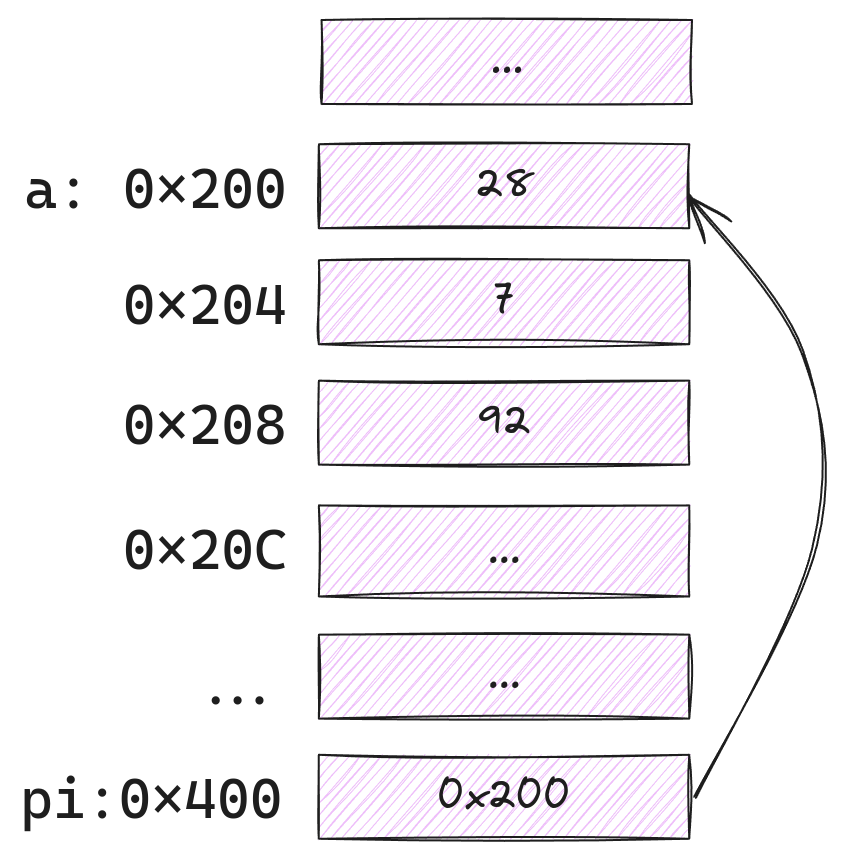
\includegraphics[width=\linewidth]{img/pointers_arith.01.png}
\end{minipage}

\vspace {0.5cm}
Notamos que el puntero \hl{pi} apunta a la dirección de memoria de \hl{a}, que es la dirección de memoria del primer elemento del array. Momento... entonces ¿qué es \hl{a}? ¿Es un puntero? ¿Es un array? \hl{a} representa un array, pero en C, un array se comporta como un puntero al primer elemento del array. Por lo tanto, \hl{a} y \hl{pi} apuntan a la misma dirección de memoria.

En la mayoría de los contextos, \hl{a} se puede usar como un puntero al primer elemento del array. Sin embargo, hay algunas diferencias importantes entre arrays y punteros que debemos tener en cuenta:
\begin{itemize}
  \item Un array tiene un tamaño fijo, mientras que un puntero puede apuntar a cualquier dirección de memoria.
  \item Un array no se puede reasignar a otra dirección de memoria, mientras que un puntero sí.
\end{itemize}
Esto significa que no podemos hacer algo como \hl{a = pi;} porque \hl{a} es un array y no se puede reasignar. Sin embargo, podemos hacer \hl{pi = a;} porque \hl{pi} es un puntero y puede apuntar a cualquier dirección de memoria.

Sigamos con el ejemplo:

\vspace {0.5cm}
\noindent
\begin{minipage}[t]{0.52\textwidth}
  \begin{cbox}[]{}
    uint32_t a[] = {28,7,92};
    uint32_t *pi = a;
    
    printf("%d\n", *pi); //28
    pi += 1;
    printf("%d\n", *pi); //7
  \end{cbox}
\end{minipage}
\hfill
\begin{minipage}[t]{0.45\textwidth}
  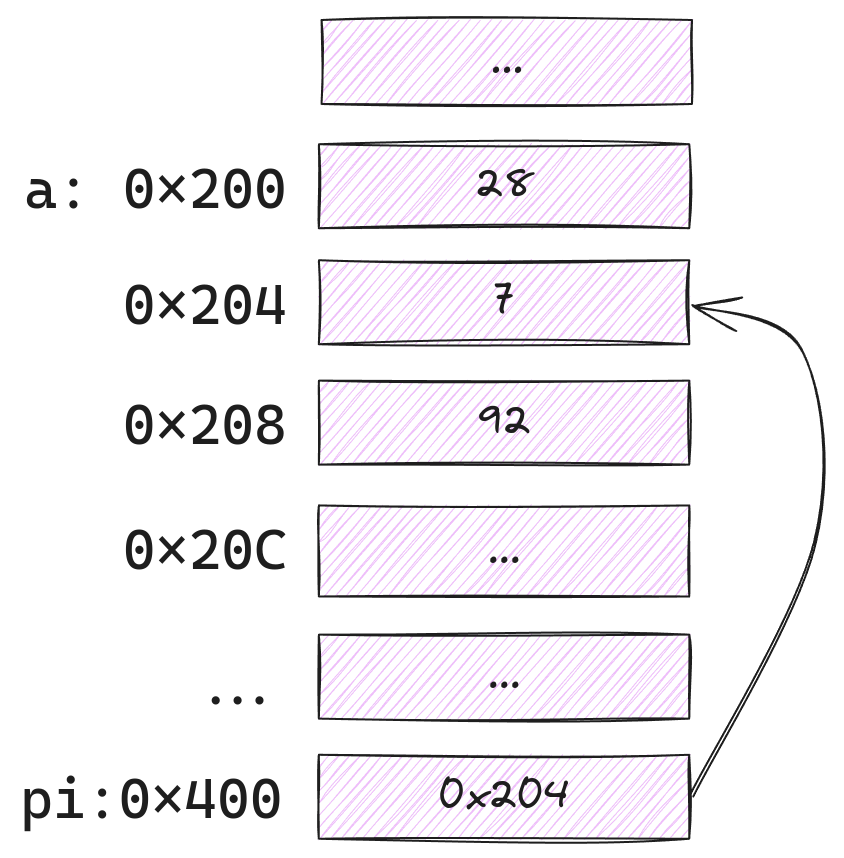
\includegraphics[width=\linewidth]{img/pointers_arith.02.png}
\end{minipage}

\vspace {1 cm}

Bien... entonces podemos usar el puntero para movernos por el array. Algo importante a notar es que la operación de ``sumar 1'', en realidad no suma 1, sino que suma el tamaño del tipo al que apunta el puntero. En este caso, \hl{pi} es un puntero a \hl{uint32\_t}, que ocupa 4 bytes. Por lo tanto, al sumar 1 a \hl{pi}, estamos sumando 4 bytes a la dirección de memoria que contiene el primer elemento del array. Esto significa que \hl{pi} ahora apunta al segundo elemento del array.

\vspace {0.5cm}

\noindent
\begin{minipage}[t]{0.52\textwidth}
  \begin{cbox}[]{}
    uint32_t a[] = {28,7,92};
    uint32_t *pi = a;
    
    printf("%d\n", *pi); //28
    pi += 1;
    printf("%d\n", *pi); //7
    pi += 1;
    printf("%d\n", *pi); //92
    
  \end{cbox}
\end{minipage}
\hfill
\begin{minipage}[t]{0.45\textwidth}
  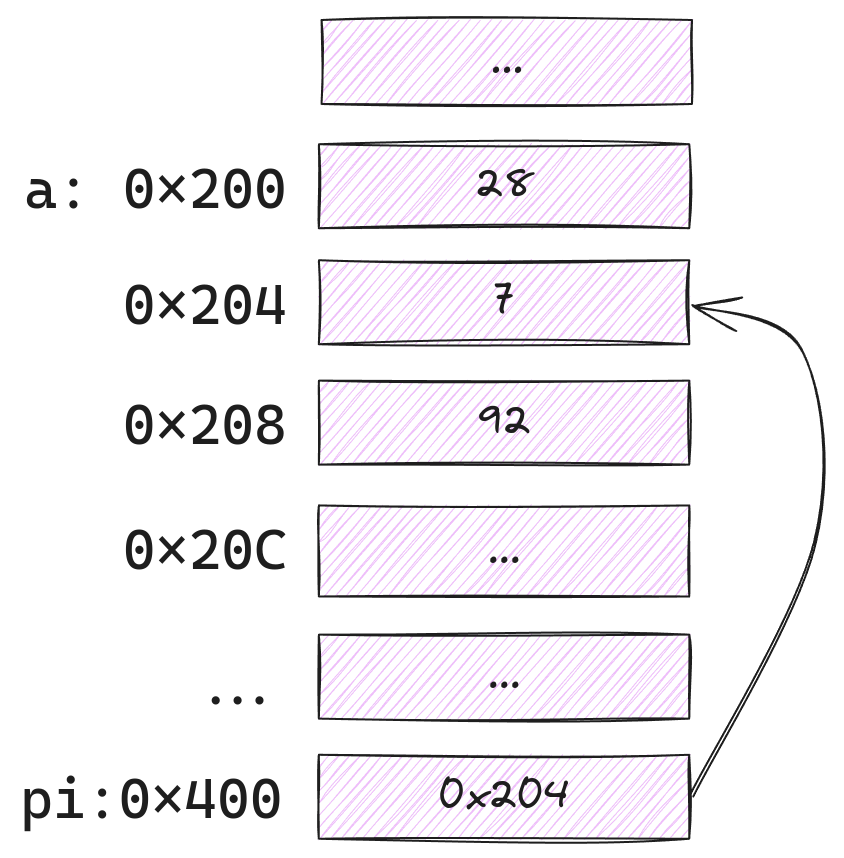
\includegraphics[width=\linewidth]{img/pointers_arith.03.png}
\end{minipage}
\vspace {0.5cm}
Ahora, si seguimos sumando 1 a \hl{pi}, llegamos al tercer elemento del array. Si seguimos sumando 1, llegaremos a la dirección de memoria que sigue al último elemento del array. Claramente, que un puntero apunte a un lugar de memoria no definido no trae ningún problema, el problema sería si queremos leer o escribir ese lugar de memoria. En ese caso, el comportamiento es indefinido, porque básicamente no sabemos que hay en esa dirección de memoria. Puede haber memoria de nuestro proceso, o puede haber memoria de otro proceso. En caso que haya memoria de otro proceso, el sistema operativo nos va a arrojar un error de \hl{Segmentation fault}. En caso que haya memoria de nuestro proceso, el comportamiento es indefinido: el programa puede seguir ejecutándose con errores lógicos o puede terminar abruptamente en un \hl{Segmentation fault}, según la operación y el tipo de memoria accedida.

Veamos otro ejemplo, para que quede claro el concepto de aritmética de punteros:

\begin{cbox}[]{}
  int arr[7] = {1,2,3,4,5,6,7};
  int *p = arr; 
  // p apunta a la dirección del primer elemento del array

  printf("%d\n", *p); // imprime 1
  printf("%d\n", *(p+1)); // imprime 2
  printf("%d\n", *(p+2)); // imprime 3
  printf("%d\n", p[4]); // imprime 5
\end{cbox}

\begin{itemize}
  \item \hl{p} es un puntero a \hl{int}, por lo tanto, al hacer \hl{p+1} estamos sumando 4 bytes a la dirección de memoria de \hl{p}
  \item al hacer \hl{p+1} estamos apuntando a la dirección de memoria del segundo elemento del array
  \item \hl{p[4]} es equivalente a \hl{*(p+4)}, es decir, estamos accediendo al quinto elemento del array
\end{itemize}

Se puede pensar el operador \hl{[]} como un operador de desreferencia. Es un \textit{shorthand} que mueve el puntero y lo desreferencia al mismo tiempo.

\begin{cbox}[]{}
p[0] == *(p+0) == *p
p[1] == *(p+1)
...
p[n] == *(p+n)
\end{cbox}

\subsection*{Punteros como argumentos}

Los punteros son útiles para pasar argumentos a funciones sin necesidad de copiar el valor completo. Esto es especialmente útil para estructuras grandes o arrays. Al pasar un puntero, estamos pasando la dirección de memoria del valor, lo que permite a la función modificar el valor original.

Aqui vemos la implementación típica de la función \hl{swap}, que intercambia los valores de dos variables enteras usando punteros:

\begin{cbox}[]{}

    void swap(int *a, int *b) {
        int tmp = *a;
        *a = *b;
        *b = tmp;
    }
    int main() {
        int x = 10, y = 20;
        swap(&x, &y);
        printf("x: %d, y: %d\n", x, y);
    }
\end{cbox}

Algo bastante común es encontrar funciones que reciben punteros como \hl{const int*} o \hl{const char*}. Esto significa que la función no puede modificar el valor al que apunta el puntero. Por ejemplo, si tenemos una función que recibe un puntero a un string, podemos usar \hl{const char*} para indicar que la función no puede modificar el string original.
Esto es útil para evitar errores de modificación accidental de datos y para indicar que la función no necesita modificar el valor. Notar que no es el puntero en sí que es constante, sino que a través de ese puntero no podemos modificar el valor al que apunta. 

\begin{exbox}
Explicar qué sucedería si la firma de la función \hl{swap} fuera \hl{void swap(int a, int b)}. En ese caso, ¿podríamos intercambiar los valores de \hl{x} e \hl{y}? 
\end{exbox}

\subsection*{Strings \textit{revisited}}

Ahora que vimos punteros, podemos ver que los strings en C son simplemente punteros a \hl{char}, terminados en \hl{\textquotesingle\textbackslash0\textquotesingle}.
Esto significa que podemos usar punteros para manipular strings de manera eficiente. Por ejemplo, podemos usar punteros para recorrer un string y modificar sus caracteres.

Tener en cuenta que los literales de strings se escriben con comillas dobles (por ejemplo, \hl{"hola"}, \hl{"f"}) y los literales de \hl{char} se escriben con comillas simples y se componen de un solo carácter (por ejemplo, \hl{'h'}, \hl{'f'}, \hl{\textquotesingle\textbackslash n\textquotesingle}).
El especificador de conversión para chars es \hl{\%c} y el de strings es \hl{\%s}. 

Veamos un ejemplo de cómo usar punteros para manipular strings:

\begin{cbox}[]{}
  #include <stdio.h>

  site_t lenght(char *str) {
      size_t len = 0;
      while (*str != '\0') {
          len++;
          str++;
      }
      return len;
  }

  int main() {
      char str[] = "This too shall pass";
      printf("Length of string: %zu\n", lenght(str));
    return 0;
  }
\end{cbox}

\begin{exbox}
Pensar si existe una diferencia entre definir un string como \hl{str1} o como \hl{str2} en el siguiente código:
\begin{cbox}[]{}
  int main(){
    char *str1 = "Hola";
    char str2[] = "Hola";

    printf("%s\n", str1);
    printf("%s\n", str2);
    return 0;
  }
  
\end{cbox}

¿Es lo mismo? Parte de la solución es pensar en la memoria. Veremos un poco más adelante como se organiza la memoria en C.
\end{exbox}

\begin{exbox}
Definir una función que reciba un string y lo pase a mayúsculas. \textbf{Pista:} alcanza con sumar la diferencia entre \hl{'A'} y \hl{'a'} a cada letra. Sólo aplicar la conversión si lo que llega es una letra minúscula. 
\end{exbox}

\begin{exbox}
Crear programas demostrativos que utilicen las funciones de strings provistas en la librería estándar de C (en \hl{string.h}): \hl{strcpy}, \hl{strcat}, \hl{strlen}, \hl{strcmp}, etc. Para acceder a la documentación de cada función se puede usar la línea de comando: \hl{man strcpy}, \hl{man strlen}, etc. 

\textbf{Side quest:} investigar que significa \hl{restrict} en la firma de la función \hl{strcpy}
\end{exbox}

\newpage
\subsection*{struct revisited}

Es normal, al declarar estructuras, querer tener un puntero al mismo tipo de estructura que estamos definiendo. Para hacer esto, lo tenemos que hacer de la siguiente manera:

\begin{cbox}[]{}
  #define NAME_LEN 50

  typedef struct persona_s {
    char nombre[NAME_LEN+1];
    int edad;
    struct persona_s* hijo;
} persona_t;
\end{cbox}

Ejemplo: Juan tiene un hijo que se llama Pablo

\begin{center}
  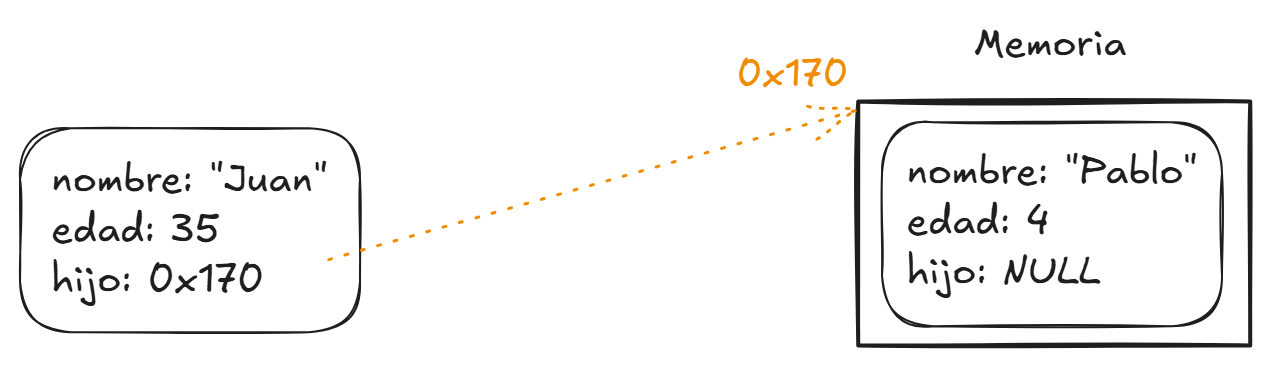
\includegraphics[scale=0.35]{./img/juan-pablo-punteros.png}  
  \captionof{table}{Juan y Pablo}
\end{center}

\begin{notebox}
  \centering
  \textbf{Nota:} usamos \hl{NULL} para indicar que Pablo no tiene hijos
\end{notebox}

Podemos crear arreglos de structs y funciones que toman structs como parámetros (o retornan structs). En este caso tenemos una función que dado un puntero a un array de \hl{persona\_t} y la longitud, imprime nombre y edad contenido en cada struct.

\begin{cbox}[unbreakable]{}
  void imprimir_personas(persona_t* personas, uint32_t longitud_array) {
      for (uint32_t i = 0; i < longitud_array; i++) {
          printf("Nombre: %s, Edad: %d\n", personas[i].nombre, personas[i].edad);
      }
  }
\end{cbox}

\newpage
\section*{Memoria}

\epigraph{\textit{Memory never recaptures reality. Memory reconstructs. All reconstructions change the original, becoming external frames of reference that inevitably fall short}}

\subsection*{Tipos de memoria}

En C tenemos varios tipos de memoria, y cada uno tiene sus propias características. Es importante entender estos tipos de memoria para poder usar C de manera efectiva. Lo que viene a continuación es bastante técnico. Quizás, una vez vistos los ejemplos que siguen, se entienda mejor.

\begin{importantbox}
  \centering
  Entender los tipos de memoria es fundamental para entender como funciona C.
\end{importantbox}

\begin{itemize}
  \item \textbf{Memoria de código}: es la memoria que se reserva para almacenar el código del programa. Su tamaño no puede cambiar durante la ejecución del programa. Es de solo lectura. Se define en el \textbf{text segment} del programa.
  \item \textbf{Memoria automática}: es un tipo de memoria que se reserva en el momento de la ejecución. Las variables locales se almacenan en esta memoria. Su tamaño puede cambiar durante la ejecución del programa. Es el llamado \textbf{stack} o pila.
    \item \textbf{Memoria estática}: es la memoria que se reserva en el momento de la compilación. Las variables globales y estáticas se almacenan en esta memoria. Su tamaño no puede cambiar durante la ejecución del programa. Se definen en el \textbf{data segment} del programa.
    \item \textbf{Memoria dinámica}: es la memoria que se reserva en el momento de la ejecución, pero su tamaño puede cambiar durante la ejecución del programa. Se utiliza para almacenar datos que no se conocen en tiempo de compilación. Es el llamado \textbf{heap}.
  \end{itemize}
  
Dependiendo de dónde y cómo declaramos nuestras variables, podremos hacer uso de una u otra memoria. Ademas de duración y scope, que vimos anteriormente, cada tipo de memoria tiene un \textbf{linkage} diferente. El linkage de un símbolo (variable o función) es la forma en que es  accesible desde diferentes archivos o módulos. 

Existen tres tipos de linkage:
\begin{itemize}
  \item \textbf{interno}: el símbolo es accesible solo dentro del archivo donde se declara.
  \item \textbf{externo}: el símbolo es accesible desde cualquier archivo que incluya su declaración.
  \item \textbf{no-linkage}: el símbolo no tiene linkage, es decir, no es accesible fuera de su scope.
\end{itemize}

La siguiente tabla muestra un panorama de los tipos de memoria, su scope, duración y linkage:

\begin{center}
  \begin{table}[!h]
    \centering
    \resizebox{\textwidth}{!}{%
      \begin{tabular}{|c|c|c|c|}
      \hline
      \rowcolor[HTML]{333333} 
      {\color[HTML]{FFFFFF} \textbf{Scope}} & {\color[HTML]{FFFFFF} \textbf{Lugar}} & {\color[HTML]{FFFFFF} \textbf{Duración}} & {\color[HTML]{FFFFFF} \textbf{Linkage}}                                    \\ \hline
      \begin{tabular}[c]{@{}c@{}}Global \\(a toda la aplicación)\end{tabular}                                        & data segment  & \begin{tabular}[c]{@{}c@{}}el tiempo de vida \\ de la aplicación (estática)\end{tabular} & externo\\ \hline
      \begin{tabular}[c]{@{}c@{}} Global \\(al archivo)\end{tabular} & data segment &
        \begin{tabular}[c]{@{}c@{}}el tiempo de vida \\ de la aplicación (estática)\end{tabular} & interno\\ \hline
        \begin{tabular}[c]{@{}c@{}}Local a la función o bloque \\(estática)\end{tabular} & data segment &
      \begin{tabular}[c]{@{}c@{}}el tiempo de vida \\ de la aplicación (estática)\end{tabular} & no linkage\\ \hline  
      \begin{tabular}[c]{@{}c@{}}Local a la función o bloque \\(automática)\end{tabular} & stack &
        \begin{tabular}[c]{@{}c@{}}Mientras la función (o bloque)\\ esté en ejecución (automática)\end{tabular} & no linkage\\ \hline
      Dinámica & heap &        
        \begin{tabular}[c]{@{}c@{}}Hasta que la memoria\\  sea liberada\end{tabular} & no linkage\\ \hline
      \end{tabular}%
    }
  \end{table}
  
\end{center}

\newpage
El linkage de una variable definida por fuera de cualquier función lo especificamos con la palabra clave \hl{static}. Esto significa que la variable no es accesible desde otros archivos, pero su duración es la misma que la de una variable global. Por lo tanto, el linkage de una variable estática es interno. Por defecto, el linkage de una variable global es externo.
Esto también aplica a funciones que tiene por defecto un linkage externo. Si queremos que una función tenga un linkage interno, debemos declararla como \hl{static}. Esto significa que la función no es accesible desde otros archivos.

Veamos ejemplos de lo anterior:

\begin{cbox}[]{archivo lib.h} 
  #ifndef LIB_H
  #define LIB_H
  
  // Idea: sólo exponer lo necesario a otros archivos

  extern int counter;        // Solo declaración, la definición está en lib.c
  void area(double radius);  // linkage externo. 
  
  #endif
\end{cbox}


\begin{cbox}[]{archivo lib.c}
  #include <stdio.h>
  #include "lib.h"

  // definición  de sólo lectura con linkage interno
  // (solo se puede usar en este archivo)
  static const double pi = 3.14159; 

  int counter = 0; // definición con linkage externo
  
  // definición con linkage interno (solo se puede usar en este archivo)
  static int power(int x) { 
      return x * x;
  }

  // definición con linkage interno (solo se puede usar en este archivo)
  static void print(double area){  
    printf("Area: %.3f\n", area);
  }
  
  void area(double radius) { // definición con linkage externo 
      double area = pi * power(radius);
      print(area);
      counter++;
  }
\end{cbox}

\begin{cbox}[]{archivo main.c}
  
  #include <stdio.h>
  #include "lib.h"

  int main() {
      double radius = 5.0;
      area(radius); // llamada a la función con linkage externo

      // acceso a la variable con linkage externo
      printf("Counter: %d\n", counter); 

      // print(3.14); // Error: no está en el header y es static en lib.c
      // power(3);    // Error: no está en el header ni tiene linkage externo
      return 0;
  }
\end{cbox}

Más información en \url{https://en.cppreference.com/w/c/language/storage_duration}.

Hemos visto hasta ahora la memoria automática y la memoria estática. La memoria automática es la que se reserva en el \textit{stack}, y la memoria estática es la que se reserva en el \textit{data segment}.
La memoria dinámica es la que se reserva en el \textit{heap}, y es la que vamos a ver a continuación.

\subsection*{Memoria dinámica}

La memoria dinámica es la que se reserva en el \textit{heap}, y es la que se utiliza para almacenar datos que no se conocen en tiempo de compilación. La memoria dinámica se reserva y libera en tiempo de ejecución, lo que permite crear estructuras de datos dinámicas como listas enlazadas, árboles, etc.

Para reservar memoria dinámica en C, usamos las funciones \hl{malloc}, \hl{calloc}, \hl{realloc} y \hl{free}. Estas funciones son parte de la biblioteca estándar de C y se encuentran en el archivo de cabecera \texttt{stdlib.h}.
\begin{itemize}
  \item \hl{malloc}: reserva un bloque de memoria de un tamaño específico y devuelve un puntero a la dirección de memoria reservada. La memoria no se inicializa.
  \item \hl{calloc}: reserva un bloque de memoria para un número específico de elementos de un tamaño específico y devuelve un puntero a la dirección de memoria reservada. La memoria se inicializa a cero.
  \item \hl{realloc}: cambia el tamaño de un bloque de memoria previamente reservado y devuelve un puntero a la nueva dirección de memoria. Si la nueva dirección es diferente, la memoria anterior se libera automáticamente.
  \item \hl{free}: libera un bloque de memoria previamente reservado.
\end{itemize}

Las declaraciones de estas funciones son las siguientes:
\begin{cbox}[]{}
  void* malloc(size_t size);
  void* calloc(size_t num, size_t size);
  void* realloc(void* ptr, size_t size);
  void free(void* ptr);
\end{cbox}

Y se encuentran en \texttt{stdlib.h}.

Analicemos un ejemplo de una función que intenta devolver un array de enteros inicializado:

\begin{cbox}[]{}
  uint16_t *secuencia(uint16_t n){
    uint16_t arr[n];
    for(uint16_t i = 0; i < n; i++)
      arr[i] = i;
    return arr;
  }
\end{cbox}

\begin{exbox}
Antes de seguir avanzando, discutan qué sucede si corren el siguiente código:
\begin{cbox}[]{}
  #include <stdio.h>

  int main(){
    uint16_t *arr = secuencia(10);
    printf("%d\n", arr[0]);
    return 0;
  }
\end{cbox}

\end{exbox}

El problema, básicamente radica en que la variable \hl{arr} es una variable automática, y por lo tanto, se libera al salir de la función. Esto significa que la dirección de memoria a la que apunta \hl{arr} ya no es válida al salir de la función. Por lo tanto, el puntero \hl{arr} en la función \hl{main} apunta a una dirección de memoria inválida.
Esto es un error común en C, y es importante tener cuidado al usar variables automáticas y punteros. Para evitar este error, podemos usar memoria dinámica para reservar el array. Veamos cómo hacerlo:
\begin{cbox}[]{}
  uint16_t *secuencia(uint16_t n){
    uint16_t *arr = malloc(n * sizeof(uint16_t));
    if (arr == NULL) {
      // Manejar el error de asignación de memoria
      return NULL;
    }
    for(uint16_t i = 0; i < n; i++)
      arr[i] = i;
    return arr;
  }
\end{cbox}

Esta función la utilizaríamos de la siguiente manera:

\begin{cbox}[]{}
  #include <stdio.h>

  int main(){
    uint16_t *arr = secuencia(10);
    if (arr == NULL) {
      // Manejar el error de asignación de memoria
      return 1;
    }
    for(uint16_t i = 0; i < n; i++)
      printf("%d\n", arr[i]);
    free(arr); // Liberar la memoria reservada
    return 0;
  }
\end{cbox}

Notemos que al usar \hl{malloc}, la memoria se reserva en el \textit{heap} y no se libera automáticamente al salir de la función. Por lo tanto, debemos liberar la memoria manualmente usando \hl{free}. Es normal que al alocación de memoria suceda en una función y la liberación en otra. Cuando nos olvidamos de liberar la memoria, se produce una \textbf{fuga de memoria} (\textit{memory leak}), que puede causar problemas de rendimiento y estabilidad en el programa. Por lo tanto, es importante liberar la memoria reservada cuando ya no la necesitamos.

\begin{exbox}
Definir una función \hl{crearPersona} que reciba un nombre y una edad, y devuelva un puntero a una estructura \hl{persona\_t} que contenga esos datos. La función debe reservar memoria dinámica para la estructura y devolver el puntero. Luego, en la función \hl{main}, crear una persona y liberar la memoria reservada.
El string que se pasa por parámetro debe ser copiado a la estructura.
\end{exbox}

\begin{exbox}
  Definir una función \hl{eliminarPersona} que reciba un puntero a una estructura \hl{persona\_t} y libere la memoria reservada para la estructura. 
\end{exbox}

\subsubsection*{Creando una lista simplemente enlazada}

Ahora, veamos un ejemplo un poco más realista. Supongamos que queremos crear una lista simplemente enlazada de nodos, donde cada nodo contiene una dirección que apunta a un archivo en un sistema de archivos determinado. La lista puede contener un número variable de nodos, con la restricción de que una lista solo puede tener nodos que apunten al mismo tipo de sistema de archivos.

Podemos ver la estructura que queremos crear en el siguiente diagrama:

\begin{center}
  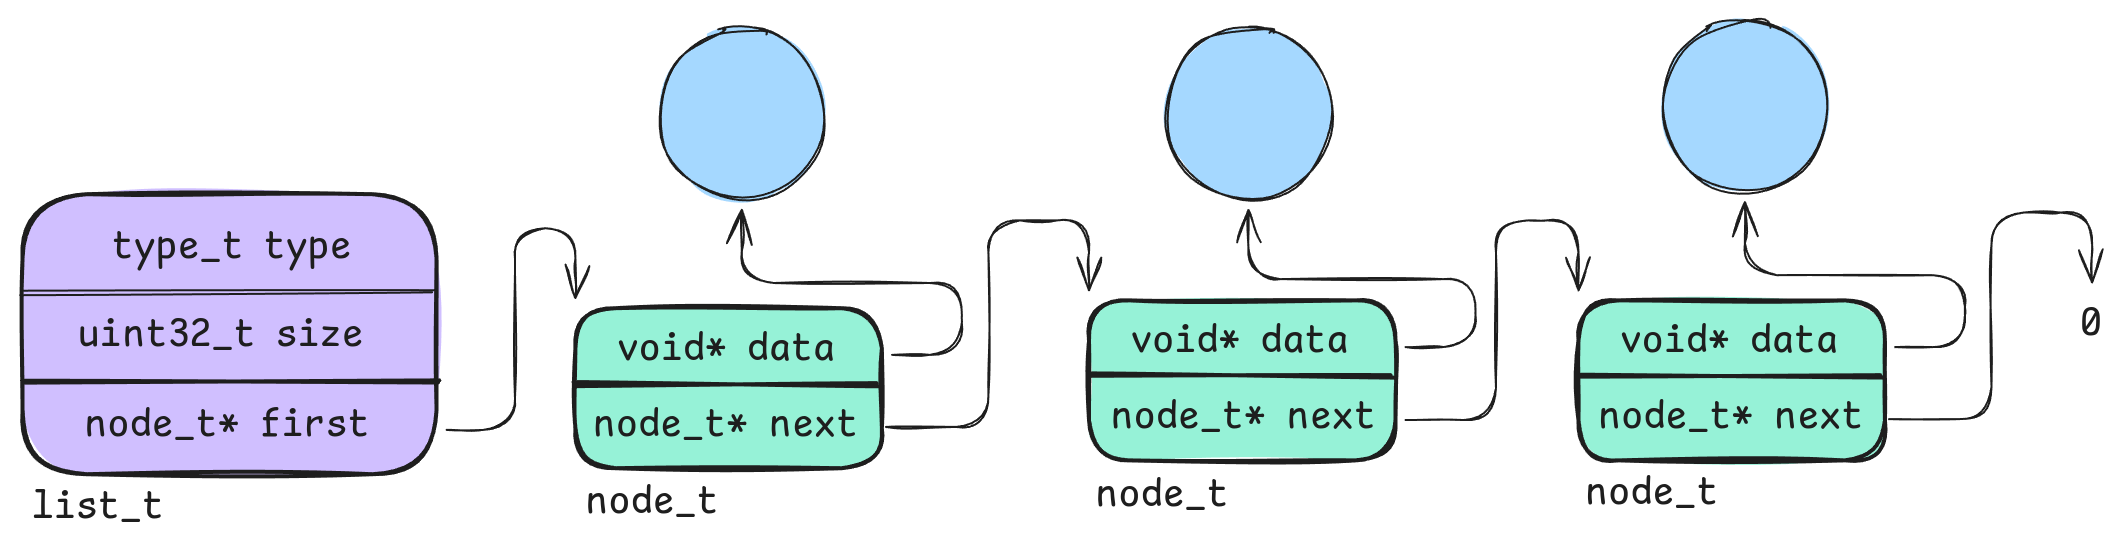
\includegraphics[scale=0.2]{./img/linkedlist.png}  
  \captionof{table}{Lista simplemente enlazada}
\end{center}

Tenemos una primera estructura que representa la lista y que tiene un puntero al primer nodo de la lista. Luego cada nodo, referencia al nodo siguiente. El último nodo apunta a \hl{NULL} para indicar el final de la lista. Cada nodo tiene un puntero a un archivo, especificado como \hl{void *data}. La lista también tiene un \hl{size} que indica la cantidad de nodos en la lista. La lista tiene un \hl{type} que indica el tipo de sistema de archivos que puede manejar esa lista. 

Veamos primero la declaración es estas estructuras:

\begin{cbox}[]{list.h}
  #include "type.h"
  
  typedef struct node {
    void* data;
    struct node* next;
  } node_t;
  
  typedef struct list {
    type_t type;
    uint8_t size;
    node_t* first;
  } list_t;

  list_t* listNew(type_t t);
  void  listAddFirst(list_t* l, void* data); //copia el dato
  void* listGet(list_t* l, uint8_t i); //se asume: i < l->size
  void* listRemove(list_t* l, uint8_t i); //se asume: i < l->size
  void  listDelete(list_t* l);

\end{cbox}

También vemos en este archivo que se declaran las funciones para crear la lista, agregar nodos, obtener nodos, eliminar nodos y eliminar la lista.
\begin{itemize}
  \item \hl{listNew} crea una nueva lista y la inicializa con el tipo de sistema de archivos especificado. La función devuelve un puntero a la lista creada.
  \item \hl{listAddFirst} agrega un nuevo nodo al principio de la lista. La función recibe un puntero a la lista y un puntero a los datos que se van a agregar. La función copia los datos en el nuevo nodo.
  \item \hl{listGet} obtiene un nodo de la lista en la posición especificada. La función recibe un puntero a la lista y un índice. La función devuelve un puntero a los datos del nodo.
  \item \hl{listRemove} elimina un nodo de la lista en la posición especificada. La función recibe un puntero a la lista y un índice. La función devuelve un puntero a los datos del nodo eliminado.
  \item \hl{listDelete} elimina la lista y libera la memoria reservada para los nodos y los datos. La función recibe un puntero a la lista.
\end{itemize}

El archivo \hl{type.h} tiene la definición de \hl{type\_t} y de las funciones de manejo de archivos para cada sistema:

\begin{cbox}[]{type.h}
  // type.h
  typedef enum e_type {
    TypeFAT32 = 0,
    TypeEXT4 = 1,
    TypeNTFS = 2
  } type_t;

  fat32_t* new_fat32();
  ext4_t* new_ext4();
  ntfs_t* new_ntfs();          
  fat32_t* copy_fat32(fat32_t* file);
  ext4_t* copy_ext4(ext4_t* file);
  ntfs_t* copy_ntfs(ntfs_t* file);
  void rm_fat32(fat32_t* file);
  void rm_ext4(ext4_t* file);
  void rm_ntfs(ntfs_t* file);
\end{cbox}

Se usa un \hl{typedef} para definir el tipo \hl{type\_t}, que es un \hl{enum} que representa los diferentes tipos de sistemas de archivos. Recordemos que un \hl{enum} es un tipo de dato que permite definir un conjunto de constantes enteras con nombre. En este caso, \hl{TypeFAT32}, \hl{TypeEXT4} y \hl{TypeNTFS} son los nombres de las constantes que representan los diferentes tipos de sistemas de archivos.

Las funciones de tipo \hl{new\_} crean archivos, y las funciones de tipo \hl{copy\_} copian archivos y las funciones de tipo \hl{rm\_} eliminan archivos. No nos interesa en este ejemplo, la definición de esas funciones, así que vamos a suponer que se encuentran en alguna biblioteca externa.

En la implementación haremos uso del operador \hl{->} y del operador \hl{sizeof}. El operador \hl{->} se usa para acceder a los miembros de una estructura a través de un puntero. Por ejemplo, \hl{l->type} accede al miembro \hl{type} de la estructura \hl{list\_t} a través del puntero \hl{l}. Esto es equivalente a \hl{(*l).type}, pero es más legible y conveniente. El operador \hl{sizeof} es una función que devuelve el tamaño en bytes de un tipo de dato o de una variable. Por ejemplo, \hl{sizeof(uint16\_t)} devuelve el tamaño en bytes del tipo \hl{uint16\_t}. Esto es útil para reservar memoria dinámica, ya que necesitamos saber cuántos bytes necesitamos reservar.

Recordar que \hl{malloc} reserva un bloque de memoria de un tamaño específico y devuelve un puntero a la dirección de memoria reservada. La memoria no se inicializa, por lo que es importante inicializarla antes de usarla.

Veamos la implementación de las funciones en el archivo \hl{list.c}:

\begin{cbox}[breakable]{list.c}
  list_t* listNew(type_t t) {
    list_t* l = malloc(sizeof(list_t));
    l->type = t;  // l->type es equivalente a (*l).type
    l->size = 0;
    l->first = NULL;
    return l;
  }

  void listAddFirst(list_t* l, void* data) {
    node_t* n = malloc(sizeof(node_t));
    switch(l->type) {
      case TypeFAT32:
        n->data = (void*) copy_fat32((fat32_t*) data);
        break;
      case TypeEXT4:
        n->data = (void*) copy_ext4((ext4_t*) data);
        break;
      case TypeNTFS:
        n->data = (void*) copy_ntfs((ntfs_t*) data);
        break;
    }
    n->next = l->first;
    l->first = n;
    l->size++;
  }

  //se asume: i < l->size
  void* listGet(list_t* l, uint8_t i){
    node_t* n = l->first;
    for(uint8_t j = 0; j < i; j++)
      n = n->next;
    return n->data;
  }

  //se asume: i < l->size
  void* listRemove(list_t* l, uint8_t i){
    node_t* tmp = NULL;
    void* data = NULL;
    if(i == 0){
      data = l->first->data;
      tmp = l->first;
      l->first = l->first->next;
    }else{
      node_t* n = l->first;
      for(uint8_t j = 0; j < i - 1; j++)
        n = n->next;
      data = n->next->data;
      tmp = n->next;
      n->next = n->next->next;
    }
    free(tmp);
    l->size--;
    return data;
  }

  void listDelete(list_t* l){
    node_t* n = l->first;
    while(n){
      node_t* tmp = n;
      n = n->next;
      switch(l->type) {
        case TypeFAT32:
          rm_fat32((fat32_t*) tmp->data);
          break;
        case TypeEXT4:
          rm_ext4((ext4_t*) tmp->data);
          break;
        case TypeNTFS:
          rm_ntfs((ntfs_t*) tmp->data);
          break;
      }
      free(tmp);
    }
    free(l);
  }
\end{cbox}

Podríamos usar la lista de la siguiente manera:

\begin{cbox}[]{main.c}
  #include <stdio.h>
  #include "list.h"

  int main() {
    list_t* l = listNew(TypeFAT32);
    fat32_t* f1 = new_fat32();
    fat32_t* f2 = new_fat32();
    listAddFirst(l, f1);
    listAddFirst(l, f2);
    listDelete(l);
    rm_fat32(f1);
    rm_fat32(f2);
    return 0;
  }
\end{cbox}

Estudien este ejemplo con detenimiento. Podemos hacer algunas optimizaciones usando punteros a función, que veremos más adelante. Por ahora, lo importante es entender cómo funcionan los punteros y la memoria dinámica en C.

\begin{exbox}
  Implementen el ejemplo anterior, implementando funciones dummy para \hl{new\_}, \hl{copy\_} y \hl{rm\_} .Pueden por ejemplo hacer usar \hl{typedef uint32\_t fat23\_t} para definir el tipo de dato \hl{fat32\_t}. Luego, en las funciones \hl{new\_} y \hl{copy\_} reservar y asignar un valor a la variable. En la función \hl{rm\_} simplemente liberar la memoria.
\end{exbox}

\begin{exbox}
  Agregar una función a la lista que permita intercambiar el orden de dos nodos. Para esto, se debe tener en cuenta que la lista puede estar vacía o tener un solo nodo. En caso de que la lista tenga un solo nodo o esté vacía, no se debe hacer nada.
\end{exbox}

\begin{exbox}
  Extender el ejemplo para que la lista sea doblemente enlazada. Esto significa que cada nodo tendrá un puntero al nodo anterior y al siguiente. Esto permitirá recorrer la lista en ambas direcciones. Para esto, se debe agregar una función para agregar un nodo al final de la lista. Mantener un puntero \hl{last} en la lista que apunte al último nodo. Esto permitirá agregar nodos al final de la lista de manera eficiente.
\end{exbox}

\subsection*{Organización de la memoria}

La memoria de un programa en C se organiza en diferentes segmentos. Cada segmento tiene un propósito específico y se utiliza para almacenar diferentes tipos de datos. La siguiente imagen muestra la organización típica de la memoria de un programa en C:

\begin{center}
  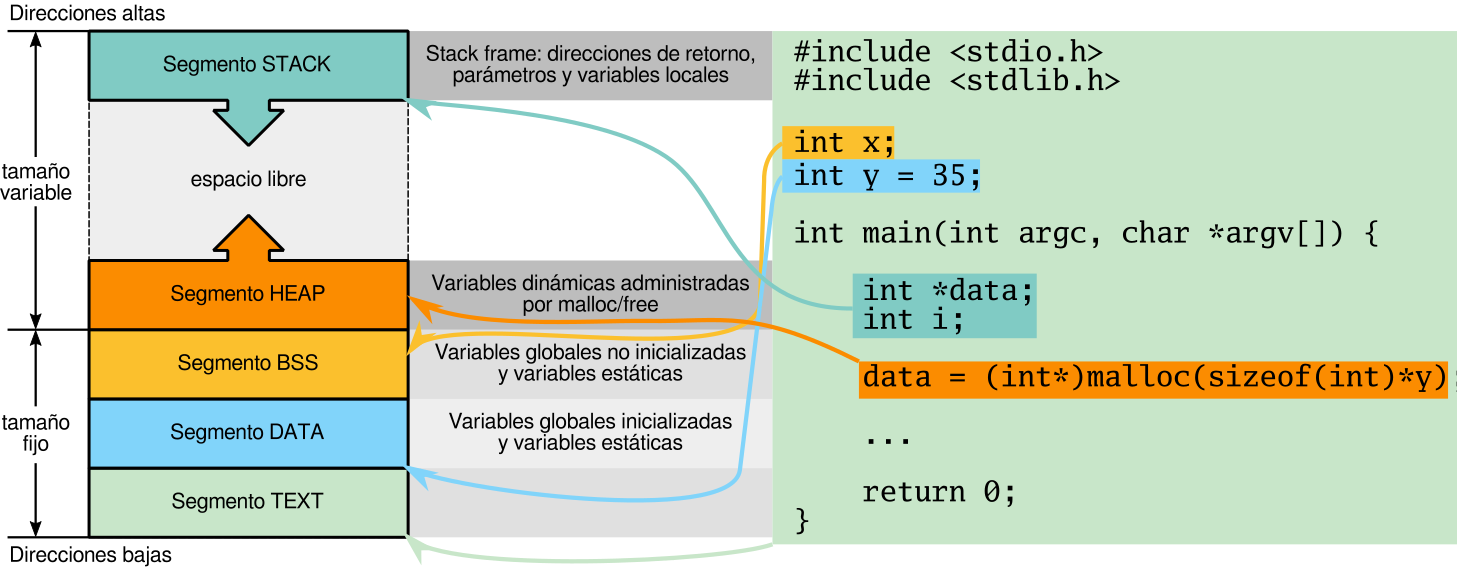
\includegraphics[scale=0.39]{./img/memory.png}  
  \captionof{table}{Imagen de memoria}
  \label{fig:memoria}
\end{center}

Cuando decimos variables globales no inicializadas, nos referimos a variables globales que no tienen un valor asignado al momento de la declaración por parte del programador. Esas variables, a diferencia de lo que sucede con las variables locales, tenemos garantías que serán inicializadas a 0. Esto es porque el compilador reserva espacio para esas variables en el segmento \textit{bss} y las inicializa a 0. Esto no sucede con las variables locales, que se reservan en el \textit{stack} y no tienen un valor asignado al momento de la declaración. Por lo tanto, su valor es indefinido.
Si inicializamos las variables globales, el compilador reserva espacio para esas variables en el \textit{data segment} y las inicializa con el valor que les asignamos. Esto es lo que sucede con las variables globales inicializadas. Las variables estáticas no globales también van a parar al \textit{data segment} o al \textit{bss} según si están inicializadas o no. 
Vemos además que la pila y el heap crecen en direcciones opuestas. Su tamaño es variable y depende del curso de ejecución que haya tomado el programa. Notar que en el diagrama tenemos el puntero \hl{data} que vive en el stack pero los datos a los que apunta, viven en el heap. Esto suele ser bastante común.

\subsection*{Problemas con memoria dinámica}

La memoria dinámica es muy útil, pero también puede ser peligrosa si no se usa correctamente. Algunos problemas comunes son:
\begin{itemize}
  \item \textbf{fugas de memoria (\textit{memory leak})}: esto sucede cuando se reserva memoria dinámica pero no se libera. Esto puede causar problemas de rendimiento y estabilidad en el programa. Para evitar esto, es importante liberar la memoria reservada cuando ya no la necesitamos.
  \item \textbf{acceso a memoria no válida (\textit{dangling pointer})}: esto sucede cuando se accede a un puntero que apunta a una dirección de memoria inválida. Esto puede causar errores de segmentación y otros problemas. 
  \item \textbf{\textit{double free}}: esto sucede cuando se libera la misma dirección de memoria dos veces. 
  \item \textbf{\textit{use after free}}: esto sucede cuando se accede a un puntero después de haber liberado la memoria a la que apunta. 
\end{itemize}

La herramienta \hl{valgrind} es muy útil para detectar estos problemas. \hl{valgrind} es una herramienta de depuración que se utiliza para detectar errores de memoria en programas. Para usar \hl{valgrind}, es recomendable compilar el programa con la opción \hl{-g} para incluir información de depuración. Luego, se puede ejecutar el programa con \hl{valgrind ./programa}. Luego de ejecutar el comando, \hl{valgrind} mostrará información sobre las fugas de memoria, accesos a memoria no válida y otros problemas de memoria. Más info en \url{https://valgrind.org/docs/manual/quick-start.html}.

\begin{exbox}
  Forzar un error de memoria en en el ejemplo de la lista enlazada, por ejemplo, al eliminar un nodo, liberar la memoria del nodo pero no liberar la memoria de los datos. Luego correr el programa con \hl{valgrind} y ver qué errores se producen.
\end{exbox}

\newpage
\section*{Punteros a punteros}
\epigraph{\textit{Not knowing what you said, you said it. }}

Hasta ahora solo usamos punteros a valores concretos, pero dado que un puntero no es más que la dirección de memoria de algún valor de algún tipo, podemos tener \textbf{punteros a cualquier cosa}.
¡Incluso podemos tener punteros a punteros!

\begin{center}
  \noindent \makebox[\textwidth]{
\includegraphics[width=0.7\paperwidth]{./img/pointing-int-meme.jpg}}
  \label{fig:pointing-int-meme}
\end{center}


Algunos ejemplos:
\begin{itemize}
  \item \hl{int**}: puntero (\texttt{int*\textcolor{red}{*}}) a un puntero a un entero (\texttt{\textcolor{red}{int*}*})
  \item \hl{void**}: puntero a puntero a un tipo \textbf{desconocido}. No se puede desreferenciar sin antes especificar su tipo mediante un \textbf{casteo}.
  \item \hl{char* argv[]}: array de punteros a \hl{char}. Esto es lo que se usa para pasar argumentos a la función \hl{main}. En este caso, \hl{argv} es un puntero a un array de punteros a \hl{char}. Es decir que cada puntero apunta a un string (un array de \hl{char}). Es lo mismo escribirlo como \hl{char** argv}\footnote{Más info en \url{https://en.cppreference.com/w/c/language/main_function}}
        
\end{itemize}

\begin{center}
  \noindent \makebox[\textwidth]{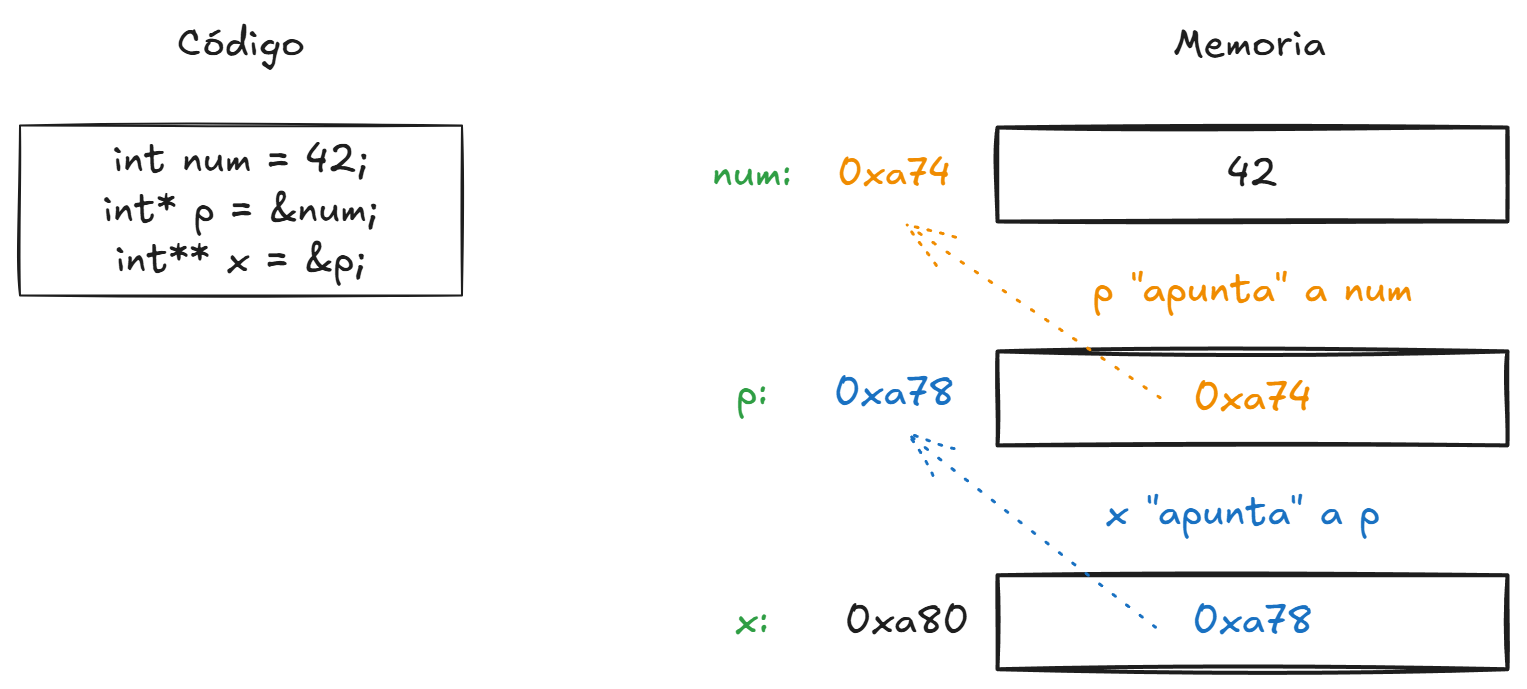
\includegraphics[width=0.7\paperwidth]{./img/puntero y doble puntero.png}}
  \label{fig:doble-puntero}
\end{center}

Analicemos el siguiente ejemplo:

\begin{cbox}[]{}
  void allocateArray(int *arr, int size, int value) {
    arr = (int*)malloc(size * sizeof(int));
    if(arr != NULL) {
      for(int i=0; i<size; i++) {
        arr[i] = value;
      }
    }
  }
  
  // Uso
  int *vector = NULL;
  allocateArray(vector,5,45);
  for(int i = 0; i < 5; i++)
    printf("%d\n", vector[i]);
  free(vector);
\end{cbox}
\begin{exbox}
  La idea de la función es alocar un array en el heap e inicializar sus valores con el valor pasado por parámetro ¿Qué sucede si corremos el código anterior? 
\end{exbox}

Lo que está pasando acá es que la función \hl{allocateArray} recibe un puntero a un entero, pero al asignar memoria a \hl{arr} dentro de la función, solo se está modificando el puntero local. Esto significa que el puntero \hl{vector} en la función \hl{main} no se ve afectado por la asignación de memoria en la función \hl{allocateArray}. Por lo tanto, al intentar acceder a \hl{vector} después de llamar a \hl{allocateArray}, se produce un error de segmentación.

La implementación correcta sería la siguiente:

\begin{cbox}[]{}
  void allocateArray(int **arr, int size, int value) {
    *arr = (int*)malloc(size * sizeof(int));
    if(*arr != NULL) {
      for(int i=0; i<size; i++) {
        (*arr)[i] = value;
      }
    }
  }
  
  // Uso
  int *vector = NULL;
  allocateArray(&vector,5,45);
  for(int i = 0; i < 5; i++)
    printf("%d\n", vector[i]);
  free(vector);
\end{cbox}


\subsection*{Arrays multidimensionales}

Los arrays multidimensionales son arrays de arrays. En C, los arrays multidimensionales se representan como punteros a punteros. Por ejemplo, un array de dos dimensiones se representa como un puntero a un puntero. 

Dado un array de dos dimensiones, definido de la siguiente manera:

\begin{cbox}[]{}
  int a[ROWS][COLS];
\end{cbox}

Podemos pensar en \hl{a} como un puntero a un puntero. En este caso, \hl{a} es un puntero a un array de \hl{COLS} enteros. Por lo tanto, \hl{a} es de tipo \hl{int (*)[COLS]}. Esto significa que \hl{a} es un puntero a un array de enteros de tamaño \hl{COLS}. Notar que ponemos el operador \hl{*} entre paréntesis para indicar que \hl{a} es un puntero a un array de enteros. Si no lo hiciéramos, \hl{a} sería un array de punteros a enteros, que no es técnicamente lo mismo.

Un array de punteros a int se vería algo así:

\begin{center}
  \noindent \makebox[\textwidth]{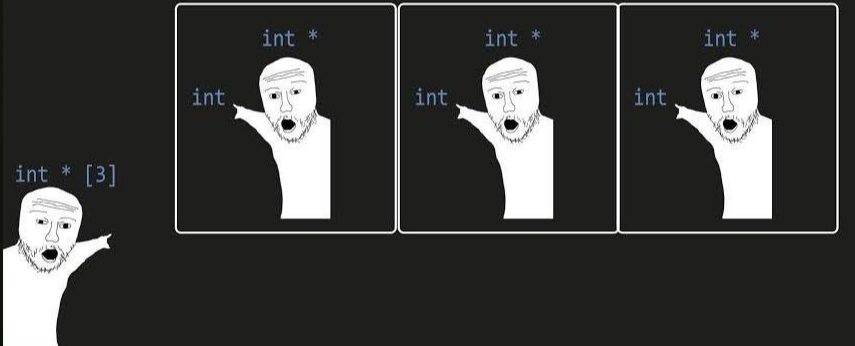
\includegraphics[width=0.6\paperwidth]{./img/array_of_pointers_meme.png}}
  \label{fig:array-of-pointers-meme}
\end{center}

Consideraciones:
\begin{itemize}
  \item Un array multidimensional es un array de arrays.
  \item La memoria se almacena de forma contigua.
  \item La notación \hl{a[i][j]} es equivalente a \hl{*(a[i] + j)}.
  \item La notación \hl{a[i][j]} es equivalente a \hl{*(a + i*COLS + j)}.
  \item El tipo de a es \hl{int (*)[COLS]}.
  \item En memoria, los arrays multidimensionales se almacenan en orden de fila (\textit{Row-major order})\footnote{\url{https://en.wikipedia.org/wiki/Row-major_order}}. Esto significa que los elementos de la primera fila se almacenan en memoria contiguamente, seguidos por los elementos de la segunda fila, y así sucesivamente.
\end{itemize}

Veamos un ejemplo:

\begin{cbox}[]{}
  int matrix[3][4] = {
    {1, 2, 3, 4},
    {5, 6, 7, 8},
    {9, 10, 11, 12}
  };

  // Todos estos prints imprimen 7
  printf("matrix[1][2]: %d\n", matrix[1][2]); 
  printf("matrix[1][2]: %d\n", *(*(matrix + 1) + 2)); 
  printf("matrix[1][2]: %d\n", *((int*) matrix + 4*1 + 2)); 

  m[0][3] = 100; // asigna 100 a la fila 0, columna 3
  printf("matrix[0][3]: %d\n", matrix[0][3]); // imprime 100
\end{cbox}  

La siguiente figura muestra el layout en memoria de dicho array:

\begin{center}
  \noindent \makebox[\textwidth]{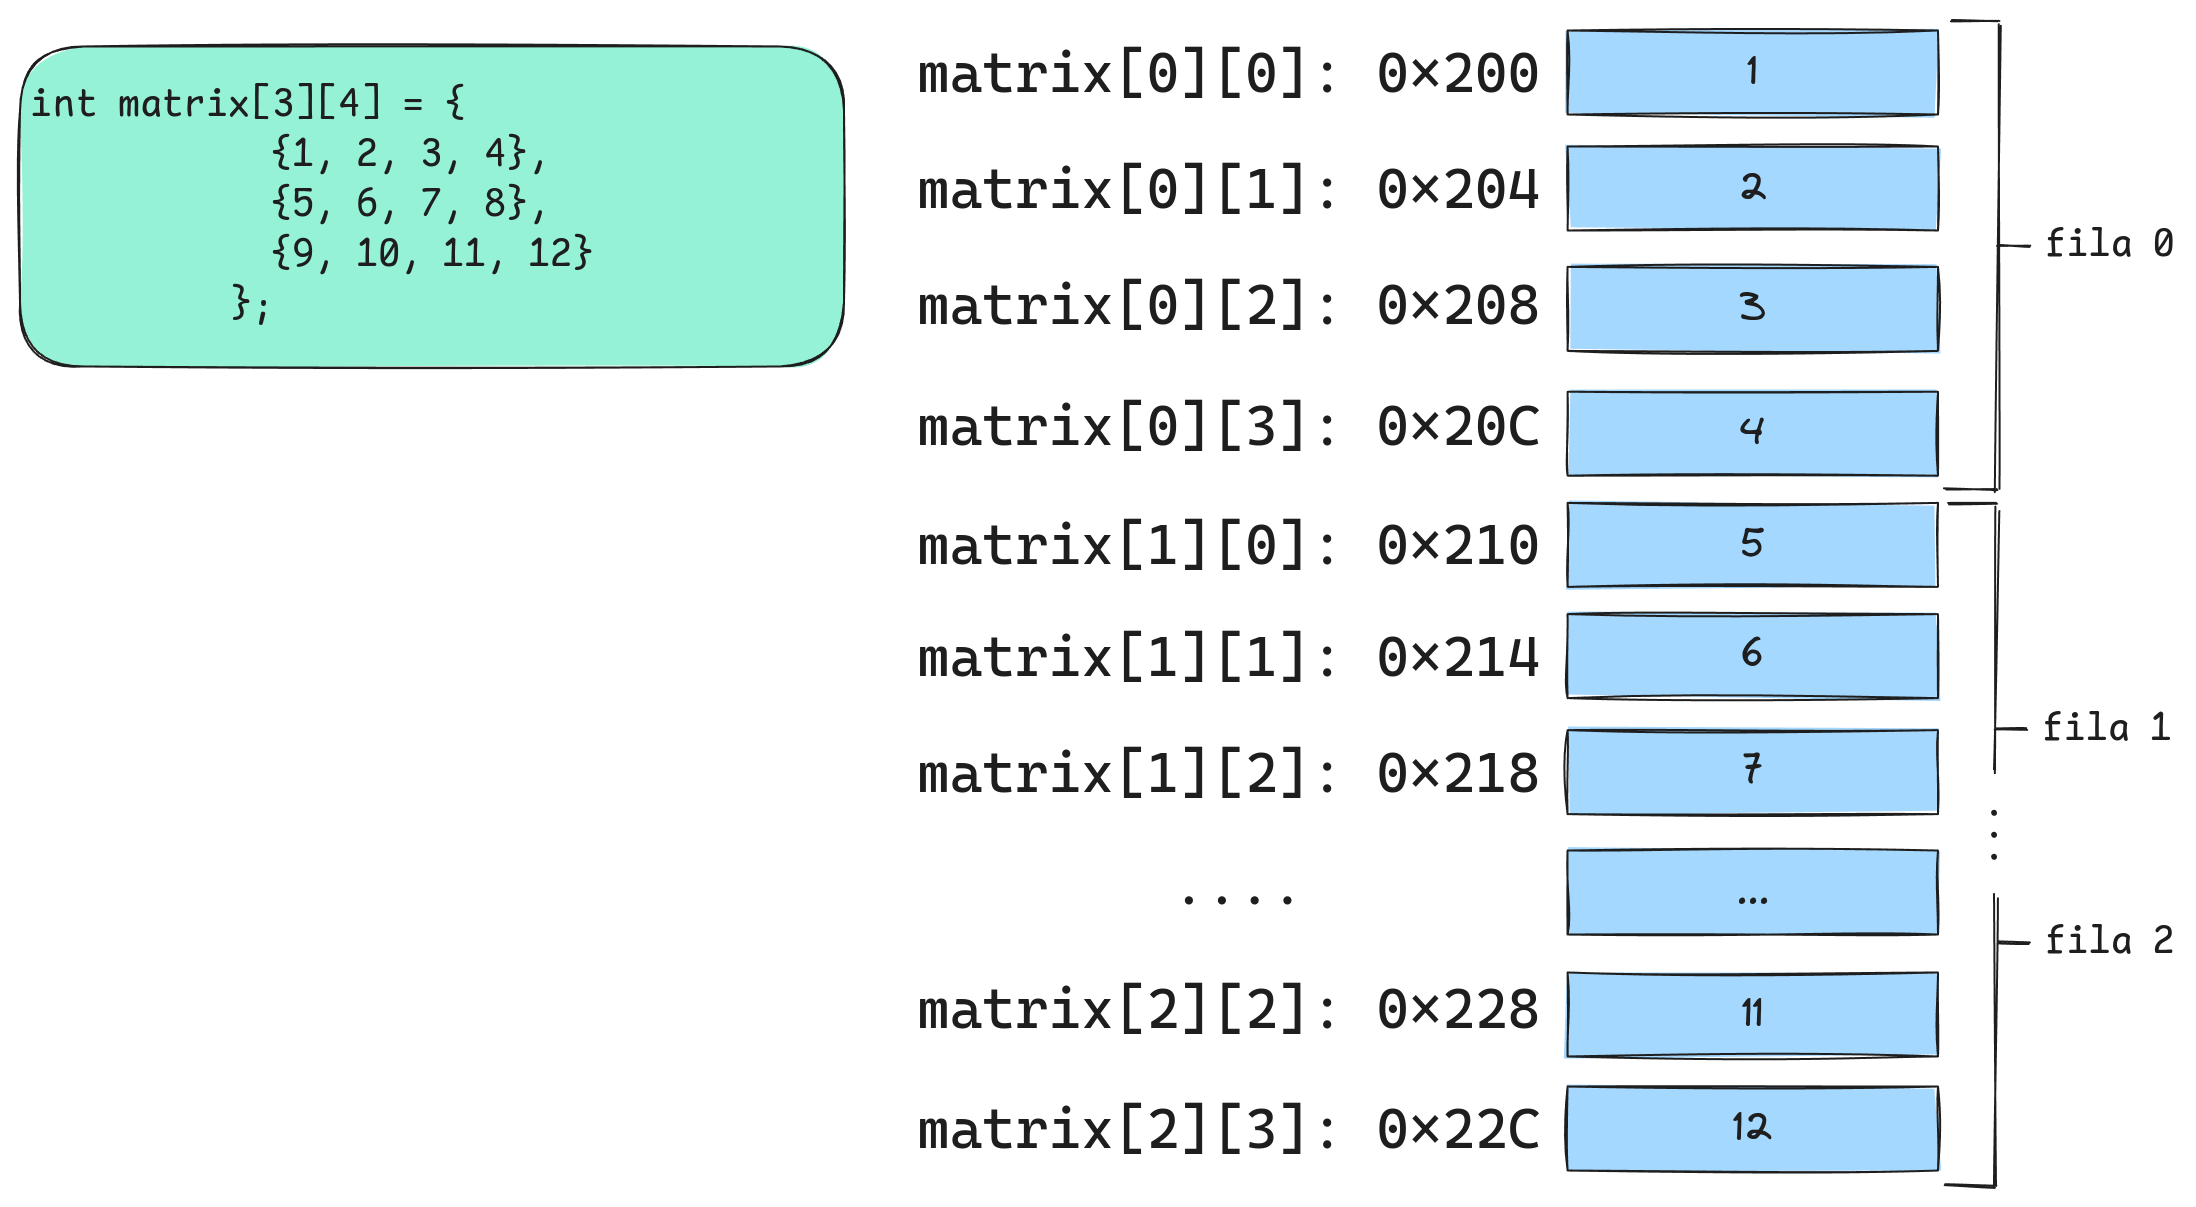
\includegraphics[width=0.7\paperwidth]{./img/arrays-multi.png}}
  \label{fig:matrix}
\end{center}

\begin{exbox}
Analicen cuidadosamente el siguiente ejemplo y respondan las preguntas:
\begin{cbox}[]{}
  #include <stdio.h>
  int main() {
      int matrix[3][4] = {
          {1, 2, 3, 4},
          {5, 6, 7, 8},
          {9, 10, 11, 12}
          };
      // p apunta al int en la fila 0, columna 0
      int *p = &matrix[0][0]; 

      // ¿qué es reshape?
      int (*reshape)[2] = (int (*)[2]) p; 

      printf("%d\n", p[3]); // Qué imprime esta línea?
      printf("%d\n", reshape[1][1]); // Qué imprime esta línea?
      return 0;
  }
\end{cbox}
\end{exbox}

\subsection*{Array de array de structs}

Analicemos ahora un caso un poco más complejo. Esto está sacado directamente del taller de system programming que veremos más adelante en la materia. 

Tenemos una posición de memoria determinada donde se aloja el buffer de vídeo. Todo lo que escribamos en ese buffer se verá reflejado en la pantalla. Recordemos que la memoria en su forma más cruda no es más que un array de bytes, como se ve a continuación:

\begin{center}
  \noindent \makebox[\textwidth]{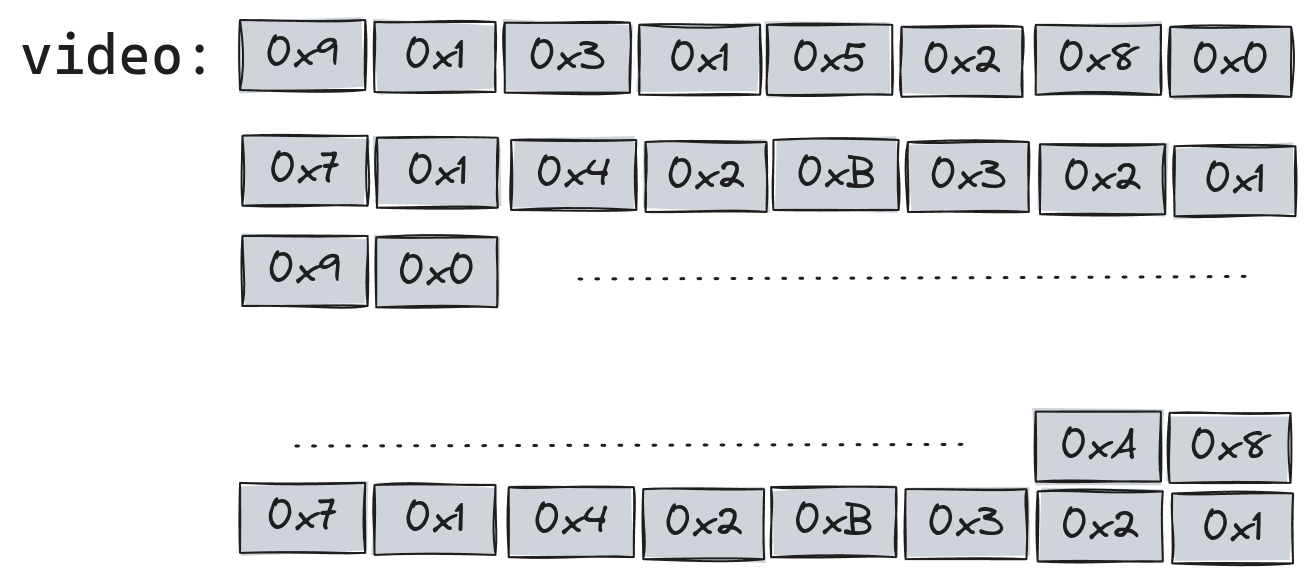
\includegraphics[width=0.7\paperwidth]{./img/videobuffer01.png}}
  \label{fig:videobuffer01}
\end{center}

El buffer de vídeo es un array de bytes y en este formato en particular, cada 2 bytes, se representa un carácter en pantalla. El primer byte representa el carácter en ascii y el segundo byte representa los atributos de color del carácter (\textit{background} y \textit{foreground}). Entonces, nos gustaría interpretar a nuestro buffer como un array de estos elementos de 2 bytes, como se ve en la siguiente figura:

\begin{center}
  \noindent \makebox[\textwidth]{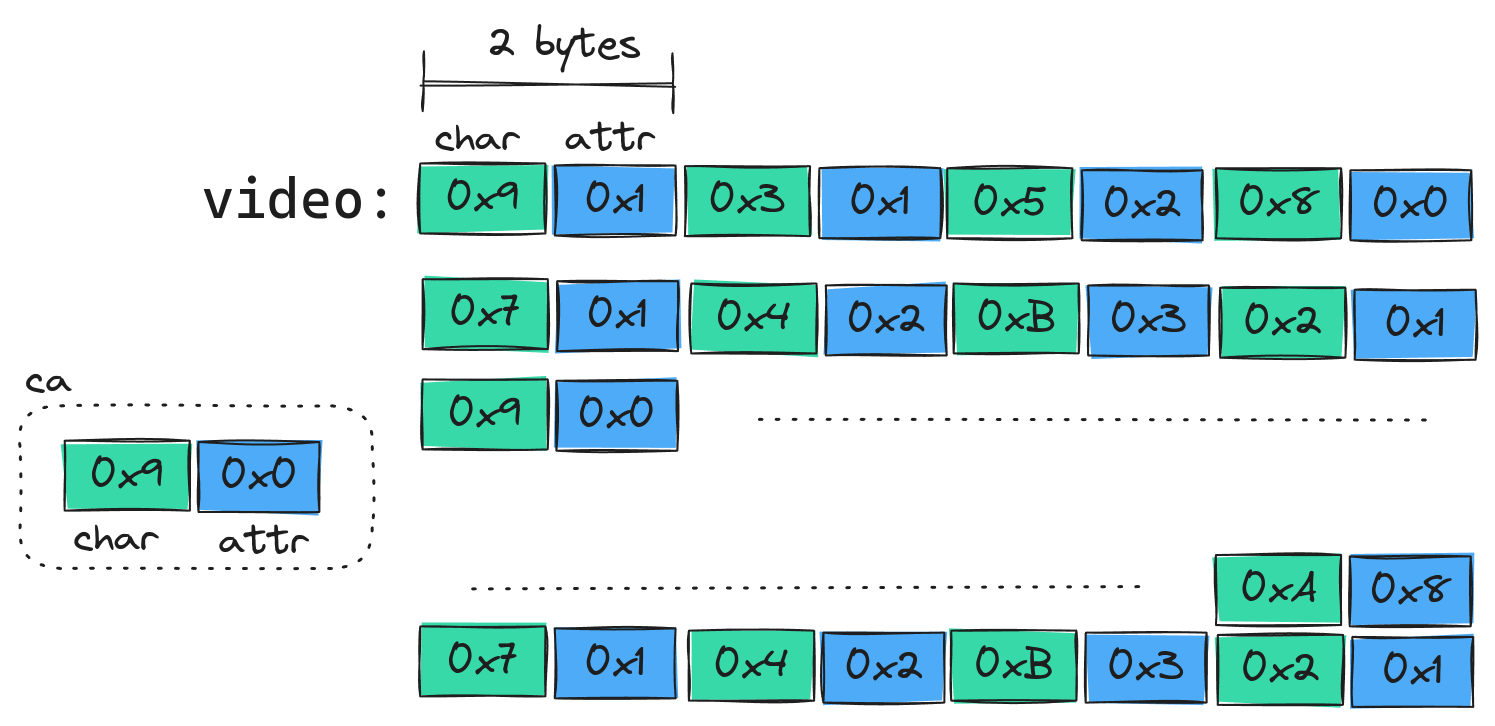
\includegraphics[width=0.7\paperwidth]{./img/videobuffer02.png}}
  \label{fig:videobuffer02}
\end{center}

En particular, como una matriz de 80x50, donde cada elemento de la matriz es un \textit{struct} que contiene el carácter y los atributos de color. 

\begin{center}
  \noindent \makebox[\textwidth]{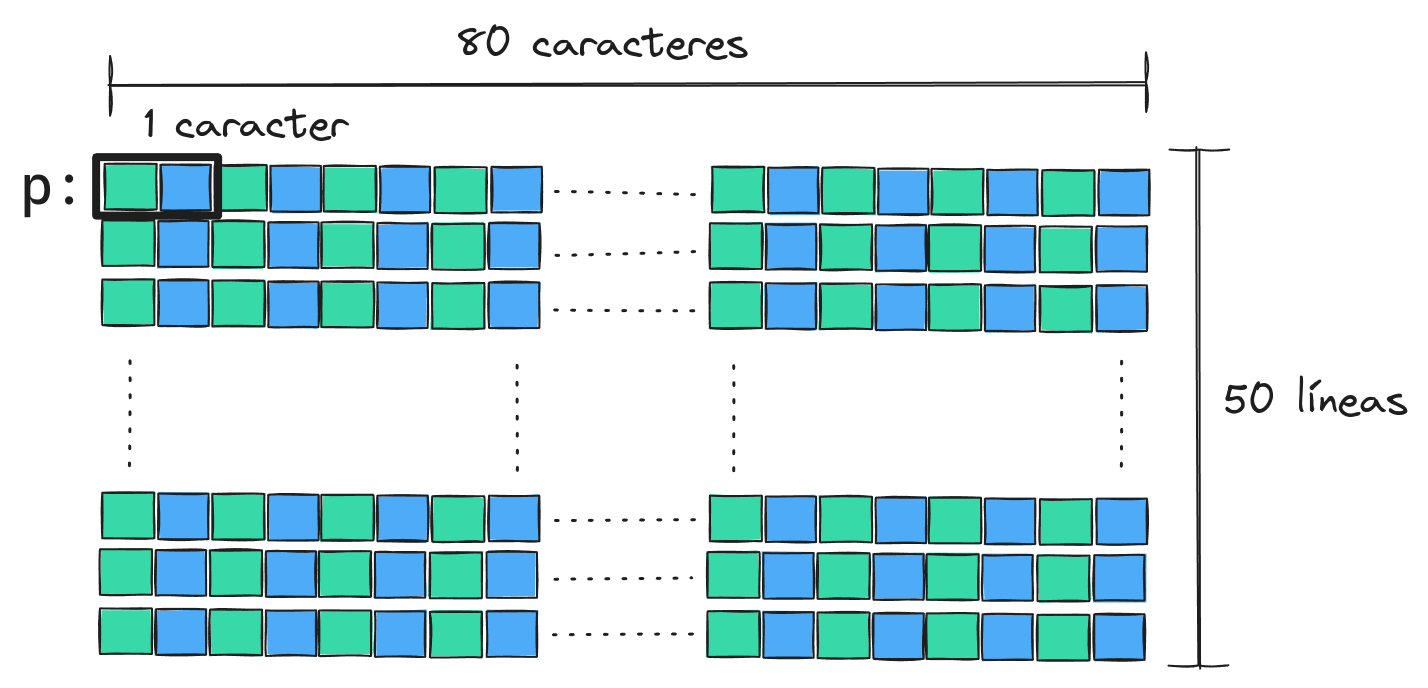
\includegraphics[width=0.7\paperwidth]{./img/videobuffer03.png}}
  \label{fig:videobuffer03}
\end{center}

El código que veremos a continuación inicializa el buffer de video:

\begin{cbox}[]{}
  #define VIDEO_COLS 80
  #define VIDEO_FILS 50
  // Cada posicion de memoria tiene 2 bytes
  typedef struct ca_s {
    uint8_t c; // caracter
    uint8_t a; // atributos
  } ca;
  void screen_draw_layout(void) {

    // VIDEO es un puntero a la dirección de memoria del buffer de video
    ca(*p)[VIDEO_COLS] = (ca(*)[VIDEO_COLS])VIDEO;
    uint32_t f,c;
    for (f = 0; f <  VIDEO_FILS; f++) {
      for (c = 0; c < VIDEO_COLS; c++) {
        p[f][c].c = ' ';
        p[f][c].a = 0x10;
      }
    }
  }
\end{cbox}

\begin{exbox}
  Analicen el código anterior y respondan las siguientes preguntas:
  \begin{itemize}
    \item ¿Qué hace \hl{ca(*p)[VIDEO\_COLS] = (ca(*)[VIDEO\_COLS])VIDEO;}?
    \item Siendo \hl{p} el puntero declarado ¿Por qué funciona esto: \hl{p[f][c].c = ' ';}? Explicar detalladamente el proceso de desreferenciación.
    \item ¿Qué pasaría si en vez de \hl{ca(*p)[VIDEO\_COLS]} hubiéramos declarado \hl{ca** p}? 
  \end{itemize}
\end{exbox}

\newpage

\section*{Punteros a función}
\epigraph{\textit{Deep in the human unconscious is a pervasive need for a logical universe that makes sense. But the real universe is always one step beyond logic.}}

Los punteros a función son punteros que apuntan a funciones en lugar de apuntar a datos. Esto permite pasar funciones como argumentos a otras funciones, lo que es útil para implementar callbacks y otras técnicas de programación avanzada.
Los punteros a función se declaran de la siguiente manera:

\begin{center}
  \begin{Verbatim}[fontshape=it]
    tipo_retorno (*nombre_puntero)(tipo_parametro1, tipo_parametro2, ...);
  \end{Verbatim}
\end{center}

Veamos algunos ejemplos de declaraciones de punteros a función: 

\begin{cbox}[]{}
  //puntero a una función que toma dos enteros y devuelve un entero
  int (*suma)(int, int);

  // puntero a una función que toma un puntero a char y devuelve void
  void (*callback)(char*);

\end{cbox}

Veamos un ejemplo sencillo de uso:

\begin{cbox}[]{puntero a función}
  #include <stdio.h>

  void print_int(int x) {
      printf("%d\n", x);
  }
  
  void pretty_print_int(int x) {
      printf("Entero[%lu bits]: %d\n", sizeof(x)*8, x);
  }
  
  int main() {
      void (*print)(int) = print_int;
      print(42);  // () desreferencia el puntero a función
      print = pretty_print_int;
      print(3);
  }
\end{cbox}

Notar como el operador \hl{()} desreferencia el puntero a función. 

Volviendo al ejemplo de la lista enlazada, podemos lograr una mayor flexibilidad al usar punteros a función para manejar los diferentes tipos de archivos. En lugar de tener un \hl{switch} en la función \hl{listAddFirst}, podemos definir un puntero a función que apunte a la función de copia correspondiente según el tipo de archivo. Esto nos permite agregar nuevos tipos de archivos sin modificar el código existente.

\begin{cbox}[]{type.h cont.}
  typedef void* (*funcCopy_t)(void*);
  typedef void (*funcRm_t)(void*);
  funcCopy_t getCopyFunction(type_t t);
  funcRm_t getRmFunction(type_t t);
\end{cbox}

Cuando vamos a devolver punteros a función, es conveniente definir un \hl{typedef} para el puntero a función. Esto hace que el código sea más legible y fácil de entender. En este caso, definimos \hl{funcCopy\_t} como un puntero a una función que toma un puntero a \hl{void} y devuelve un puntero a \hl{void}. También definimos \hl{funcRm\_t} como un puntero a una función que toma un puntero a \hl{void} y no devuelve nada.

\begin{cbox}[]{list.c cont.}
  funcCopy_t getCopyFunction(type_t t) {
    switch (t) {
        case TypeFAT32: return (funcCopy_t) copy_fat32; break;
        case TypeEXT4:  return (funcCopy_t) copy_ext4; break;
        case TypeNTFS:  return (funcCopy_t) copy_ntfs; break;
        default: return NULL; break;
    }
  }
  
  funcRm_t getRmFunction(type_t t) {
    switch (t) {
        case TypeFAT32: return (funcRm_t) rm_fat32; break;
        case TypeEXT4:  return (funcRm_t) rm_ext4; break;
        case TypeNTFS:  return (funcRm_t) rm_ntfs; break;
        default: return NULL; break;
    }
\end{cbox}

Entonces podemos modificar las funciones \hl{listAddFirst} y \hl{listDelete} para usar los punteros a función:

\begin{cbox}[]{list.c cont.}
  void listAddFirst(list_t* l, void* data) {
    node_t* n = malloc(sizeof(node_t));
    n->data = getCopyFunction(l->type)(data);
    n->next = l->first;
    l->first = n;
    l->size++;
  }

  void listDelete(list_t* l){
    node_t* n = l->first;
    while(n){
      node_t* tmp = n;
      n = n->next;
      getRmFunction(l->type)(tmp->data);
      free(tmp);
    }
    free(l);
  }
\end{cbox}

\begin{exbox}
  Agregar las modificaciones necesarias al ejemplo de la lista enlazada para usar punteros a función.
\end{exbox}

\subsubsection*{Declaraciones confusas}

Todo es risas y diversión hasta que nos encontramos con declaraciones siniestras como las siguientes:

\begin{cbox}[]{}
  // puntero a función que toma dos punteros a double y devuelve un puntero 
  // a un array de 10 double
  double (*(*f3)(double*, double*))[10];

  // puntero a función que toma un puntero a char y devuelve un puntero a 
  // función que toma un puntero a int y devuelve void
  void (*(*f4)(char*))(int*);
\end{cbox}

\begin{center}
  \noindent \makebox[\textwidth]{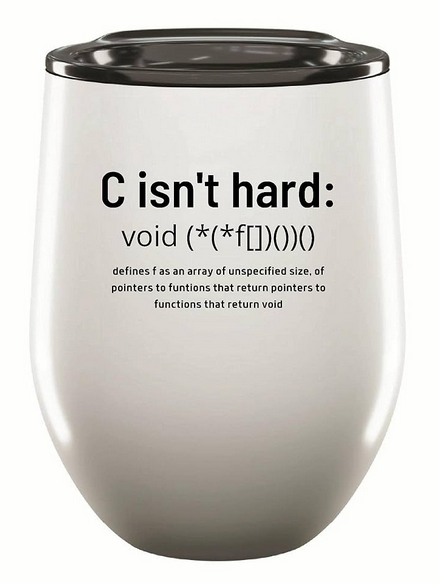
\includegraphics[width=0.4\paperwidth]{./img/function-pointer-meme.png}}
  \label{fig:function-pointer-meme}
\end{center}

Pueden visitar el sitio \url{https://cdecl.org/} para ver declaraciones y su interpretación en inglés. En general las declaraciones pueden volverse más manejables con los \hl{typedef} correspondientes.

\begin{cbox}[]{}
  // definimos primero f3_t, como un puntero a función tradicional
  typedef double DoubleArray10[10];
  typedef DoubleArray10* DoubleArray10Ptr;
  typedef DoubleArray10Ptr (*f3_t)(double*, double*);

  // y luego declaramos f3 de tipo f3_t
  f3_t f3;
  

  // definimos primero InnerFunc, como un puntero a función tradicional
  //  que toma un puntero a int y devuelve void
  typedef void InnerFunc(int*);

  // luego, definimos primero f4_t, como un puntero a función tradicional
  //  que toma  un puntero a char y devuelve un puntero a InnerFunc
  typedef InnerFunc* (*f4_t)(char*);
  
  // finalmente, declaramos f4 de tipo f4_t
  f4_t f4;
\end{cbox}

\newpage
\section*{Anexo: Ejemplo integrador}
\epigraph{\textit{Intelligence takes chance with limited data in an arena where mistakes are not only possible but also necessary.}}

Como ejemplo integrador vamos a definir algunas operaciones sobre listas enlazadas en C.

Una lista enlazada es una estructura de datos donde cada nodo contiene un valor y un puntero al siguiente nodo de la lista. La lista $[1,2,3]$ se puede pensar de la siguiente manera:

\begin{center}
  \noindent \makebox[\textwidth]{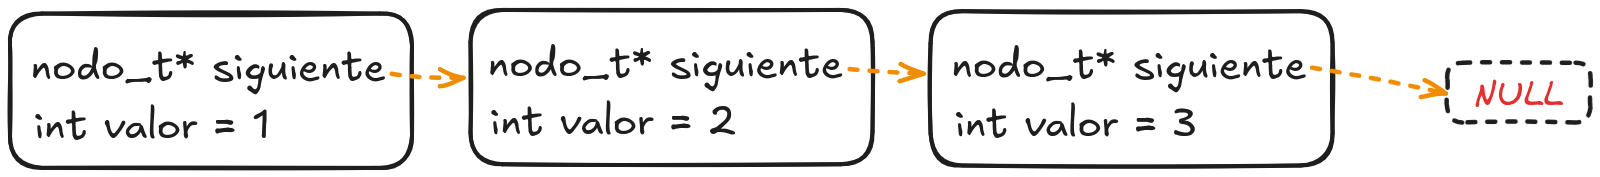
\includegraphics[width=0.8\paperwidth]{img/lista_enlazada.png}}
  \label{fig:linked-list}
\end{center}

El primer nodo de una lista se denomina la \textbf{cabeza} de la lista. Una lista se recorre comenzando por la cabeza y avanzando al siguiente nodo hasta que no haya un siguiente nodo al cual avanzar.

Primero tenemos que definir las estructuras que van a representar a la lista enlazada en memoria. Para esto vamos a definir dos structs, \hl{lista\_t} para representar el la lista en sí misma y \hl{nodo\_t} para los elementos que forman la lista.

\begin{cbox}[unbreakable]{declaración de estructuras de lista enlazada}
typedef struct nodo_s {
    // hay que definir struct nodo_s* acá porque el tipo nodo_t 
    // no está declarado.
    struct nodo_s* siguiente;
    int valor;
} nodo_t;

typedef struct lista_s {
    nodo_t* cabeza;
} lista_t;
\end{cbox}

Una \hl{lista\_t} está definida por el puntero a la cabeza de la lista, es decir el primer nodo de la lista. Luego en cada \hl{nodo\_t} se almacena el valor que este representa y el puntero al siguiente nodo en la lista (si es que dicho nodo existe).

Primero vamos a definir funciones pare crear una lista vacía y un nuevo nodo.

\begin{cbox}[unbreakable]{}
lista_t* crear_lista_vacia() {
    lista_t* lista_vacia = malloc(sizeof(lista_t));
    lista_vacia->cabeza = NULL; // El operador x->y es equivalente a (*x).y
    return lista_vacia;
}

nodo_t* crear_nuevo_nodo(int valor) {
    nodo_t* nuevo_nodo = malloc(sizeof(nodo_t));
    nuevo_nodo->siguiente = NULL;
    nuevo_nodo->valor = valor;
    return nuevo_nodo;
}
\end{cbox}

Estas funciones crean una lista vacía y un nodo respectivamente, retornan un puntero a la estructura creada. Ambas estructuras se encuentran en el \textit{heap}.

¿Por qué tenemos que reservar memoria con \hl{malloc} para crear una lista vacía o un nuevo nodo? Pensemos en esta otra implementación (errónea) de \hl{crear\_nuevo\_nodo}:

\begin{cbox}[unbreakable]{}
nodo_t* crear_nuevo_nodo_incorrecto(int valor) {
    nodo_t nuevo_nodo; // Esta estructura se almacena en el stack.
    nuevo_nodo.siguiente = NULL;
    nuevo_nodo.valor = valor;
    return &nuevo_nodo; // Retornamos una dirección de memoria del stack.
}
\end{cbox}

En esta implementación el nuevo nodo se define en el stack. Esa porción de memoria es válida durante todo el tiempo de vida del \textit{stack frame}, es decir hasta el momento que retorna la función. Luego cualquier acceso a ese puntero estaría escribiendo o leyendo en una dirección de memoria que probablemente le corresponda al \textit{stack frame} de otra función. \textbf{Evitar este tipo de errores en C queda a criterio del programador. Hay instancias en las que se pueden cometer errores de memoria similares a este y que el programa aparente funcionar bien.}

Ahora con estas funciones podemos definir otras operaciones típicas en listas enlazadas, como agregar elementos al final:

\begin{cbox}[unbreakable]{}
void insertar_al_final(lista_t* lista, int valor) {
    nodo_t* actual = lista->cabeza;
    nodo_t* a_insertar = crear_nuevo_nodo(valor);

    // Caso lista vacia. 
    // Intentar desreferenciar el puntero NULL causa un 
    // Segmentation Fault (SIGSEGV).
    if (actual == NULL) {
        lista->cabeza = a_insertar;
        return;
    }

    while (actual->siguiente != NULL)
        actual = actual->siguiente;

    actual->siguiente = a_insertar;
}
\end{cbox}

A diferencia de otros lenguajes en C no hay excepciones\footnote{Esto quiere decir que operaciones que en otros lenguajes, como Python, levantan un error en C pasan desapercibidas a menos que se haga un chequeo explícito. Por ejemplo en Python si $lista = [1,2,3]$, la operación $lista[5]$ levanta una excepción. En C nada nos impide indexar un array fuera de rango.}. Una convención que se suele usar es que una función retorne un código de error indicando si la operación tuvo éxito o no. Por ejemplo podemos escribir una función que borre la cabeza de una lista. Retorna 0 si pudo borrar la cabeza de la lista y retorna -1 si la lista ya estaba vacía:

\begin{cbox}[unbreakable]{}
int eliminar_cabeza(lista_t* lista) {
    nodo_t* actual = lista->cabeza;
    if (actual == NULL)
        return -1;
    lista->cabeza = actual->siguiente;
    free(actual);
    return 0;
}
\end{cbox}

Notar que esta función una vez que acomoda la lista con la nueva cabeza, llama a \hl{free} con el puntero a la anterior cabeza. Esto es necesario pues ese es el último momento en el que el puntero a la cabeza original es alcanzable dentro de algún \textit{scope}. En C si no se indica explícitamente, nunca se libera memoria reservada con \hl{malloc}. Hay que tener cuidado de no llamar a \hl{free} antes de estar seguros de que nadie va a querer usar la porción de memoria referenciada. En programas más complejos esto se puede solucionar, por ejemplo, manteniendo un contador de referencias activas.

Siguiendo este razonamiento podemos escribir una función que borre la lista completa:
\begin{cbox}[unbreakable]{}
void eliminar_lista(lista_t* lista) {
    nodo_t* actual = lista->cabeza;
    while (actual != NULL) {
        nodo_t* siguiente = actual->siguiente;
        free(actual);
        actual = siguiente;
    }
    free(lista);
}
\end{cbox}

Como último ejemplo vamos a definir la función \hl{map} sobre listas de números enteros. La función \hl{map} recibe como parámetro un puntero a una \hl{lista\_t} y un puntero a una función de la forma \hl{int (*operacion)(int)}. Esto quiere decir un puntero a una función, llamada \hl{operacion} en este caso, que toma como único argumento un \hl{int} y retorna un \hl{int}. Luego \hl{map} modifica la lista aplicando la función \hl{operacion} a cada uno de sus elementos. 
Por ejemplo:
$$
f(x) = 2x
$$
$$
map([1,2,3,4,5], f) = [2,4,6,8,10]
$$

\newpage %nueva página para no cortar función map

\begin{cbox}[unbreakable]{}
void map(lista_t* lista, int (*operacion)(int)) {
    nodo_t* actual = lista->cabeza;
    while (actual != NULL) {
        actual->valor = operacion(actual->valor);
        actual = actual->siguiente;
    }
}
\end{cbox}

Ejemplo de uso:

\begin{cbox}[unbreakable]{}
int duplicar(int x) {
    return x*2;
}

int main() {
    lista_t* mi_lista = crear_lista_vacia();
    insertar_al_final(mi_lista, 1);
    insertar_al_final(mi_lista, 2);
    insertar_al_final(mi_lista, 3);
    insertar_al_final(mi_lista, 4);
    // En este momento mi_lista = [1,2,3,4]
    map(mi_lista, &duplicar);
    // En este momento mi_lista = [2,4,6,8]
    eliminar_lista(mi_lista);
    return 0;
}
\end{cbox}

Como ejercicio opcional pueden probar implementar la función \hl{filter} que elimina de \hl{lista} todos los elementos en los que \hl{criterio} evalúa a 0. En la página siguiente hay una posible implementación, de todos modos recomendamos que intenten escribir una propia antes de consultarla.
\begin{bashbox}[minted language=C]
void filter(lista_t* lista, int (*criterio)(int));
\end{bashbox}

Un posible criterio podría ser:
\begin{cbox}[unbreakable]{}
int es_par(int x) {
    if (x % 2 == 0)
        return 1;
    else
        return 0;
}
\end{cbox}

\newpage

Esta es una posible solución al problema, no es la única, ni la más compleja, ni la más sencilla:

\begin{cbox}[unbreakable]{}
void filter(lista_t* lista, int (*criterio)(int)) {
    nodo_t** cabeza_actual = &lista->cabeza;
    while (*cabeza_actual != NULL) {
        if (!criterio((*cabeza_actual)->valor)) {
            nodo_t* a_borrar = *cabeza_actual;
            *cabeza_actual = (*cabeza_actual)->siguiente;
            free(a_borrar);
        } else {
            cabeza_actual = &(*cabeza_actual)->siguiente;
        }
    }
}
\end{cbox}

Parece bastante razonable, si la cabeza de la lista no cumple con el criterio, la borro y continúo operando con la sub-lista que me queda. No importa que esté en el primer elemento, el décimo o el último. Pero... ¿Qué está pasando con \hl{cabeza\_actual}? \\

Primero empezamos por el tipo, \hl{cabeza\_actual} es un puntero a un puntero a \hl{nodo\_t}. Esto quiere decir que es una dirección de memoria que apunta a otra dirección de memoria, y esta última apunta a un \textit{struct} de tipo \hl{nodo\_t}. Al principio se inicializa en la dirección de memoria en la que reside el campo \texttt{cabeza} de la lista, este campo es de tipo \hl{nodo\_t*}, por lo que nos queda algo de tipo \hl{nodo\_t**}. \\

Vamos a ver en detalle las primeras iteraciones para la lista $[1,2,3,4,5,..., k]$ para el predicado \texttt{es\_par} dado como ejemplo en el enunciado del ejercicio. \\

La convención de coloreo en los dibujos para los tipos representados es: \\

\begin{center}
  \noindent \makebox[\textwidth]{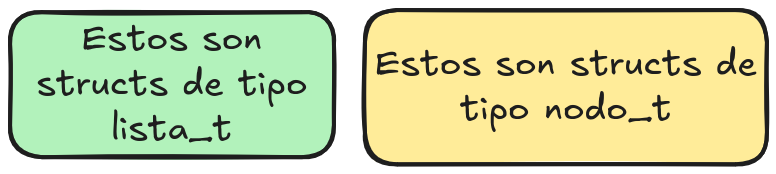
\includegraphics[width=0.4\paperwidth]{img/referencia.png}}
\end{center}

\newpage

\texttt{Paso 0:} Antes de entrar al ciclo, inicializamos \hl{cabeza\_actual} en el principio de la lista.

\begin{center}
  \noindent \makebox[\textwidth]{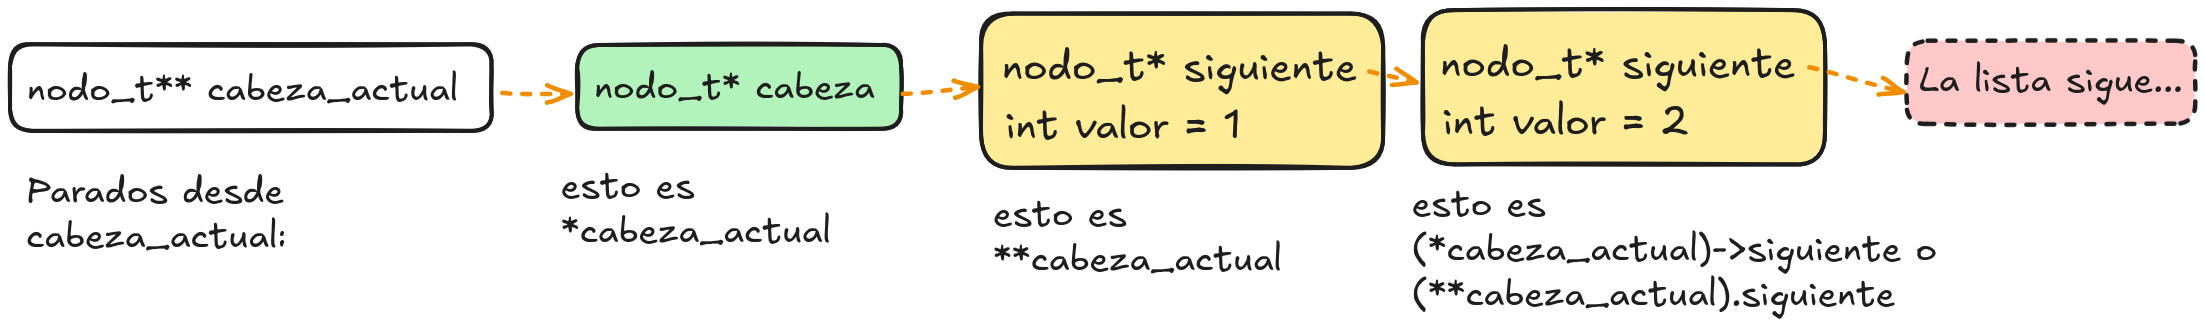
\includegraphics[width=0.8\paperwidth]{img/init.png}}
\end{center}

\texttt{Paso 1:} Borrar el 1 de la lista y avanzar al siguiente elemento.

\begin{center}
  \noindent \makebox[\textwidth]{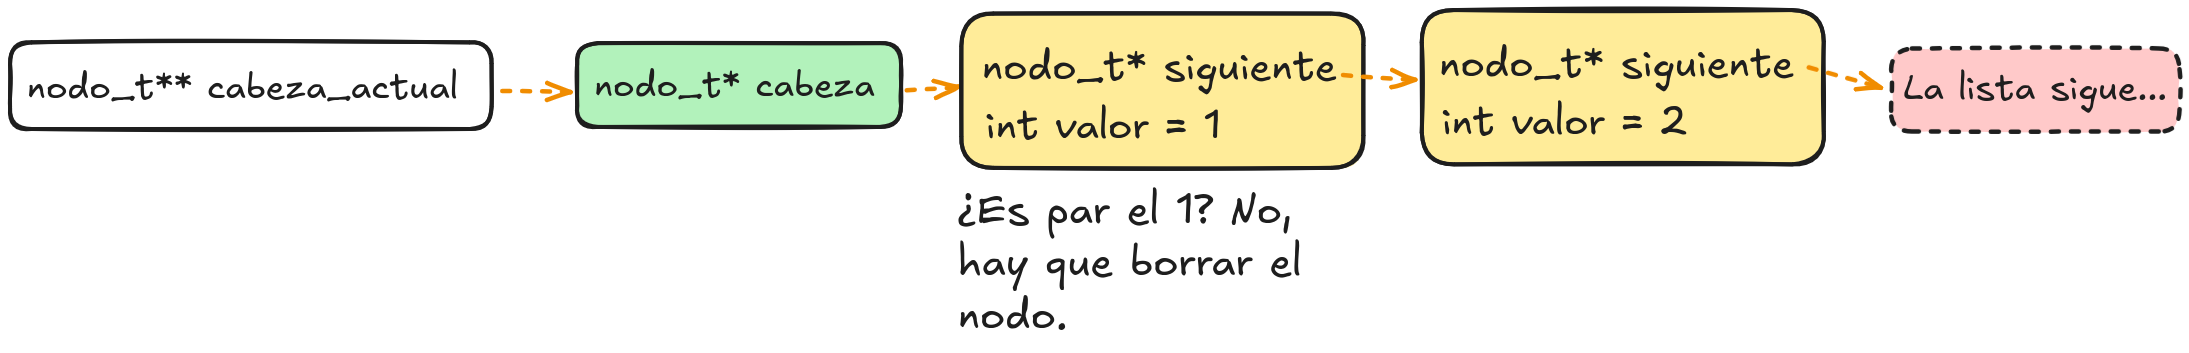
\includegraphics[width=0.8\paperwidth]{img/iter1.png}}
\end{center}

Antes de pasar al paso 2 está sucediendo esto:
\begin{bashbox}[minted language=C]
    nodo_t* a_borrar = *cabeza_actual;
    *cabeza_actual = (*cabeza_actual)->siguiente;
    free(a_borrar);
\end{bashbox}

\texttt{Paso 2:} Preservar el 2 y avanzar al siguiente elemento. 

\begin{center}
  \noindent \makebox[\textwidth]{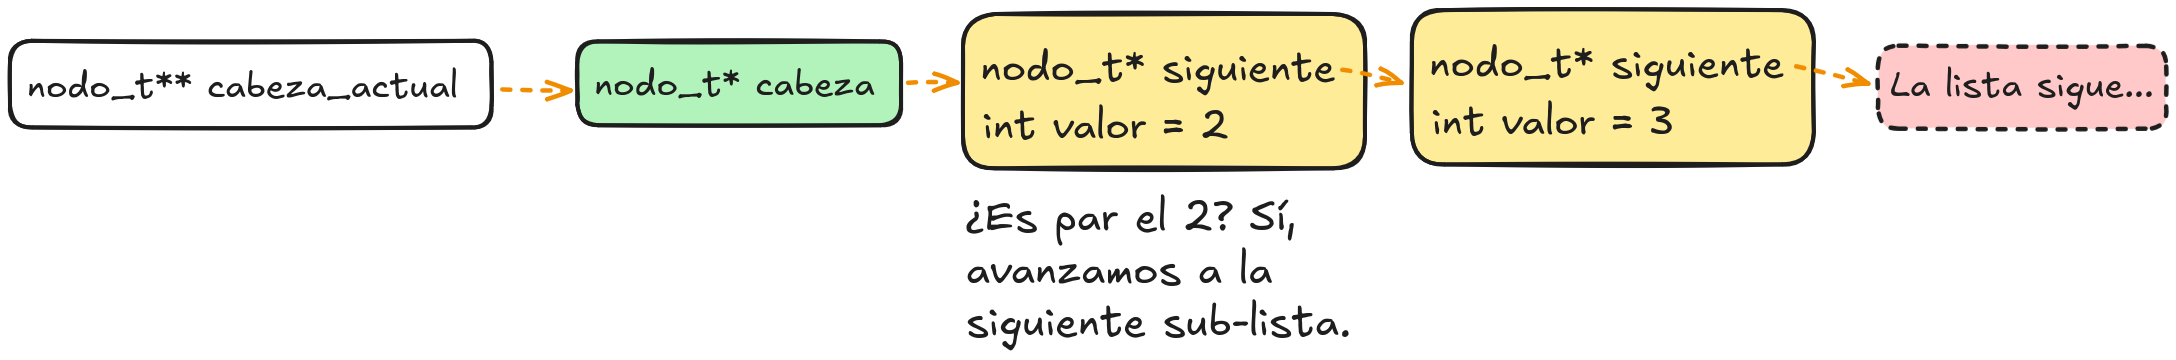
\includegraphics[width=0.8\paperwidth]{img/iter2.png}}
\end{center}

Antes de pasar al paso 3 está sucediendo esto:
\begin{bashbox}[minted language=C]
    cabeza_actual = &(*cabeza_actual)->siguiente;
\end{bashbox}

\texttt{Paso 3:} Borrar el 3 de la lista y avanzar al siguiente elemento.

\begin{center}
  \noindent \makebox[\textwidth]{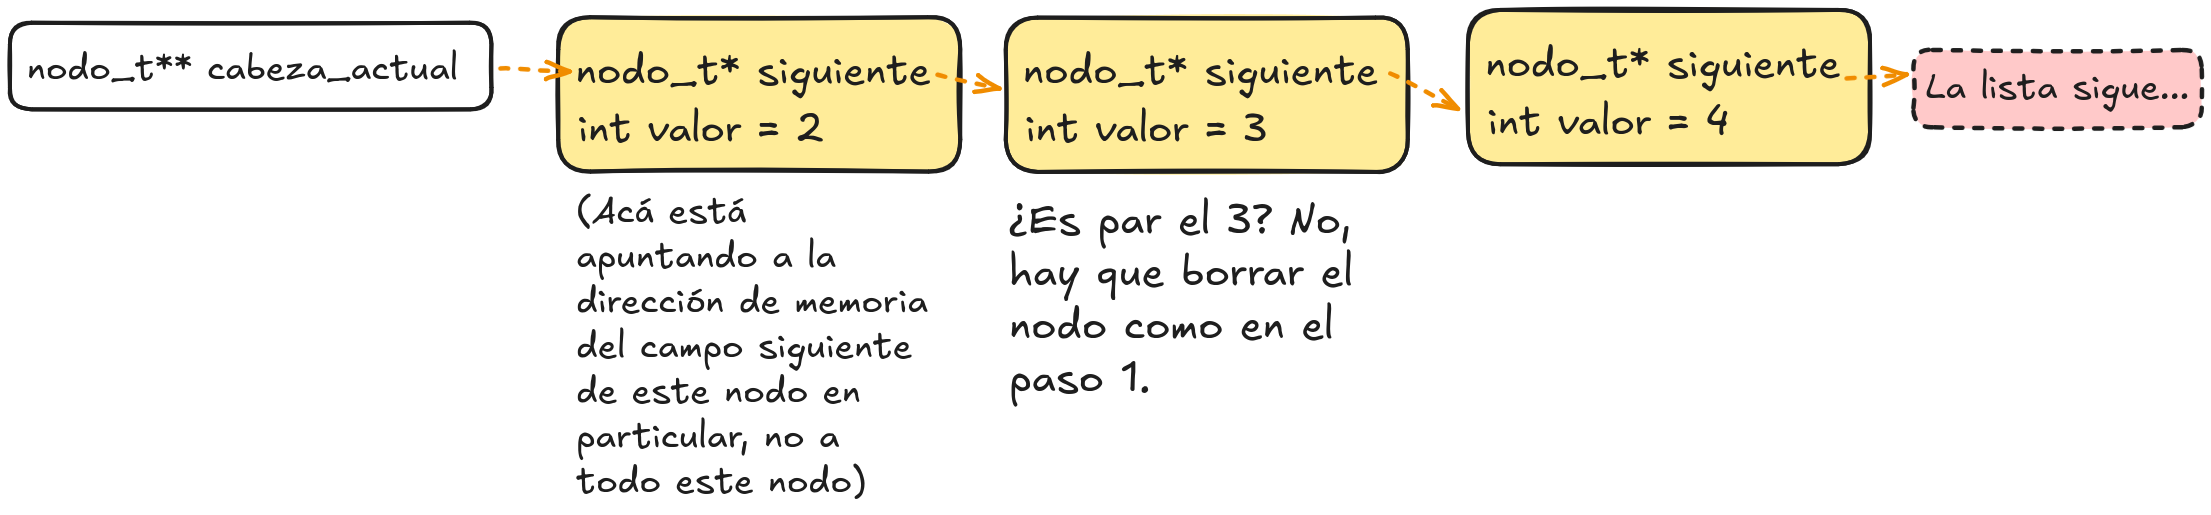
\includegraphics[width=0.8\paperwidth]{img/iter3.png}}
\end{center}
\texttt{Paso 4:} Preservar el 4 y avanzar al siguiente elemento. 

\begin{center}
  \noindent \makebox[\textwidth]{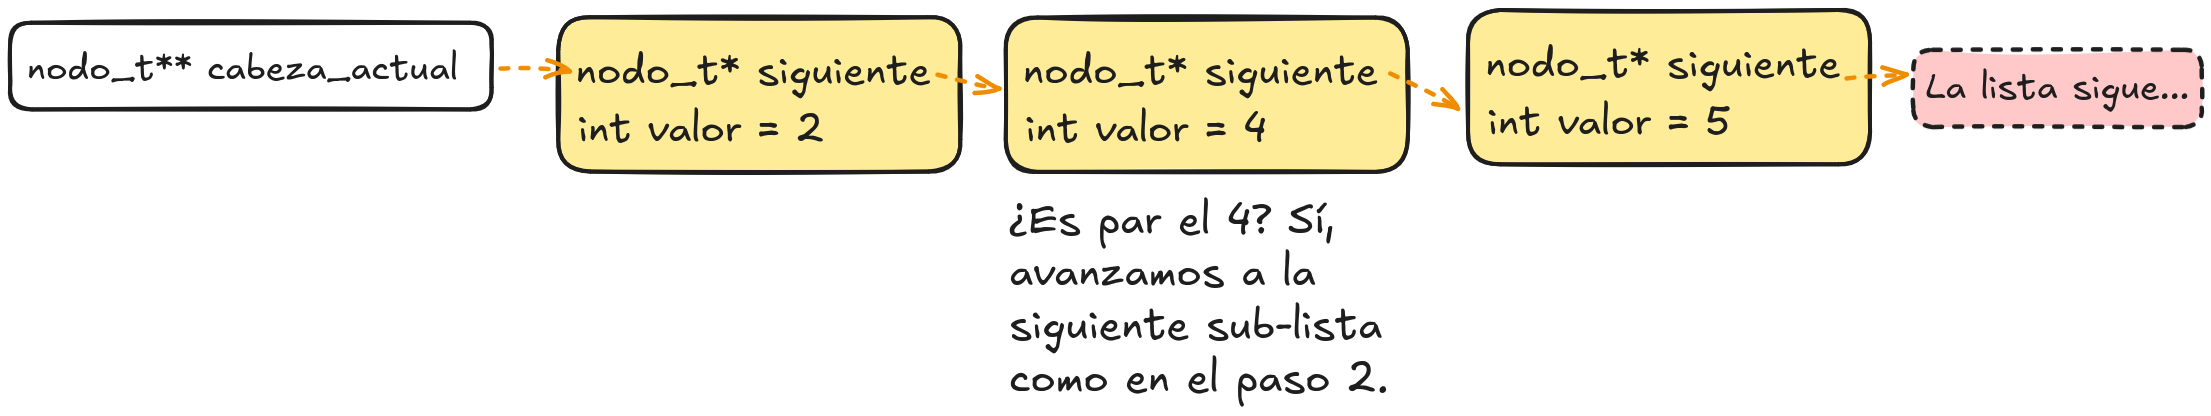
\includegraphics[width=0.8\paperwidth]{img/iter4.png}}
\end{center}

Esto continúa hasta llegar al final de la lista, donde \hl{*cabeza\_actual} va a ser igual a \hl{NULL} y no se entra al ciclo.

\newpage
\section*{Referencias}

\epigraph{\textit{Most believe that a satisfactory future requires a return to an idealized past, a past which never in fact existed.}}

\begin{itemize}
  \item Kernighan, Ritchie - The C Programming Language, 2nd Edition.
  \item Seacord, Robert - Effective C: An Introduction to Professional C Programming 
  \item C reference: \url{https://en.cppreference.com/w/c }
  \item GNU C reference: \url{https://gcc.gnu.org/onlinedocs/gcc/}
  \item Valgrind documentation: \url{https://valgrind.org/docs/manual/quick-start.html}
  \item Cdecl: \url{https://cdecl.org/}
  \item C programming: \url{https://www.learn-c.org/}
\end{itemize}

\end{document}
